\subsection{Caso d'uso UC9: Gestione dei questionari}
\label{UC9}
\begin{figure}[h]
	\centering
	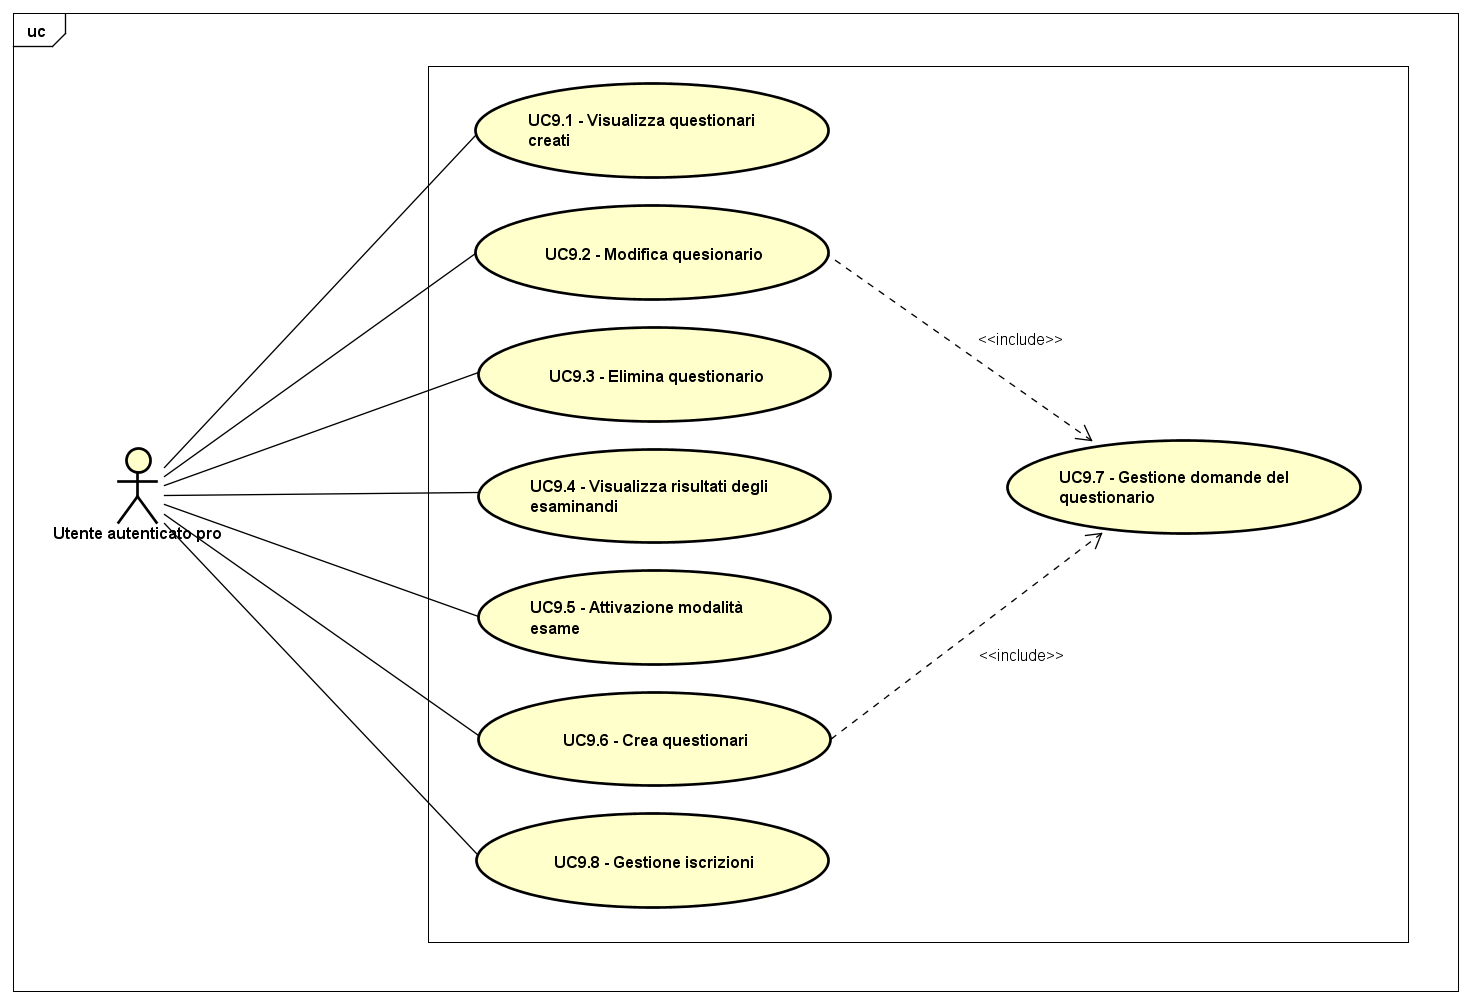
\includegraphics[scale=0.7,keepaspectratio]{UML/UC9.png}
	\caption{UC9: Gestione dei questionari}
\end{figure}
\FloatBarrier
\begin{itemize}
	\item \textbf{Attori}: 
	\item \textbf{Descrizione}: 
	\item \textbf{Precondizione}: 
	\item \textbf{Postcondizione}: 
	\item \textbf{Scenario principale}:
	\item \textbf{Inclusioni}:
	\item \textbf{Estensioni}:
	\item \textbf{Scenari alternativi}:
\end{itemize}

	\subsubsection{Caso d'uso UC9.1: Visualizza questionari}
	\label{UC9.1}
	\begin{figure}[h]
		\centering
	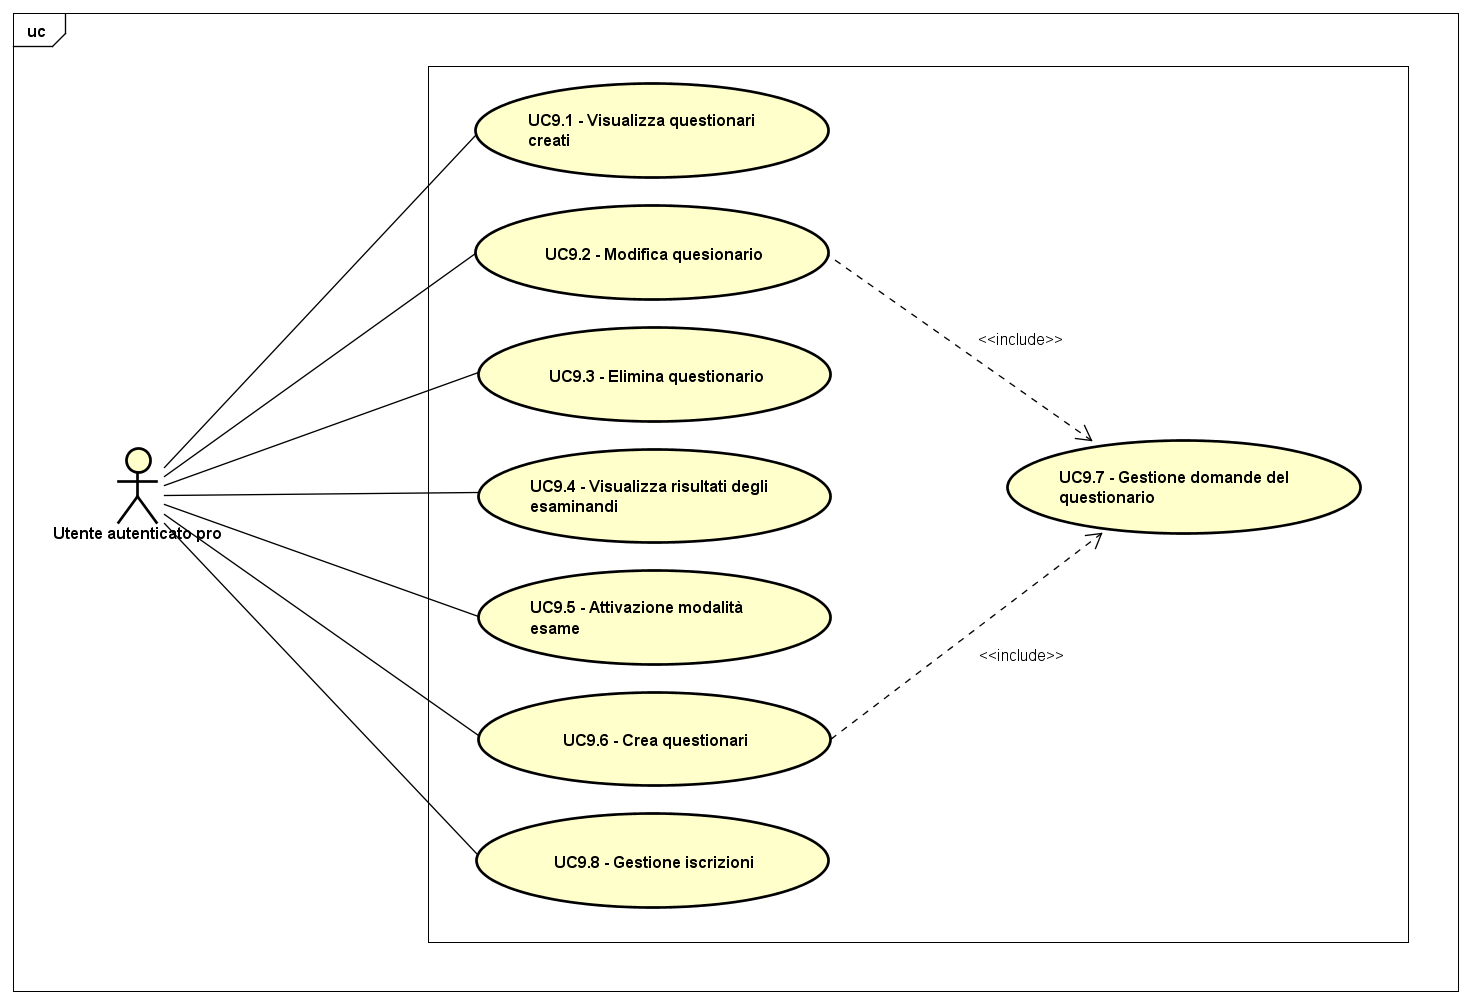
\includegraphics[scale=0.7,keepaspectratio]{UML/UC9.png}
		\caption{UC9.1: Visualizza questionari}
	\end{figure}
	\FloatBarrier
	\begin{itemize}
		\item \textbf{Attori}: 
		\item \textbf{Descrizione}: 
		\item \textbf{Precondizione}: 
		\item \textbf{Postcondizione}: 
		\item \textbf{Scenario principale}:
		\item \textbf{Inclusioni}:
		\item \textbf{Estensioni}:
		\item \textbf{Scenari alternativi}:
	\end{itemize}
	
		\paragraph{Caso d'uso UC9.1.1: Visualizza questionari preferiti}
		\label{UC9.1.1}
		\begin{figure}[h]
			\centering
		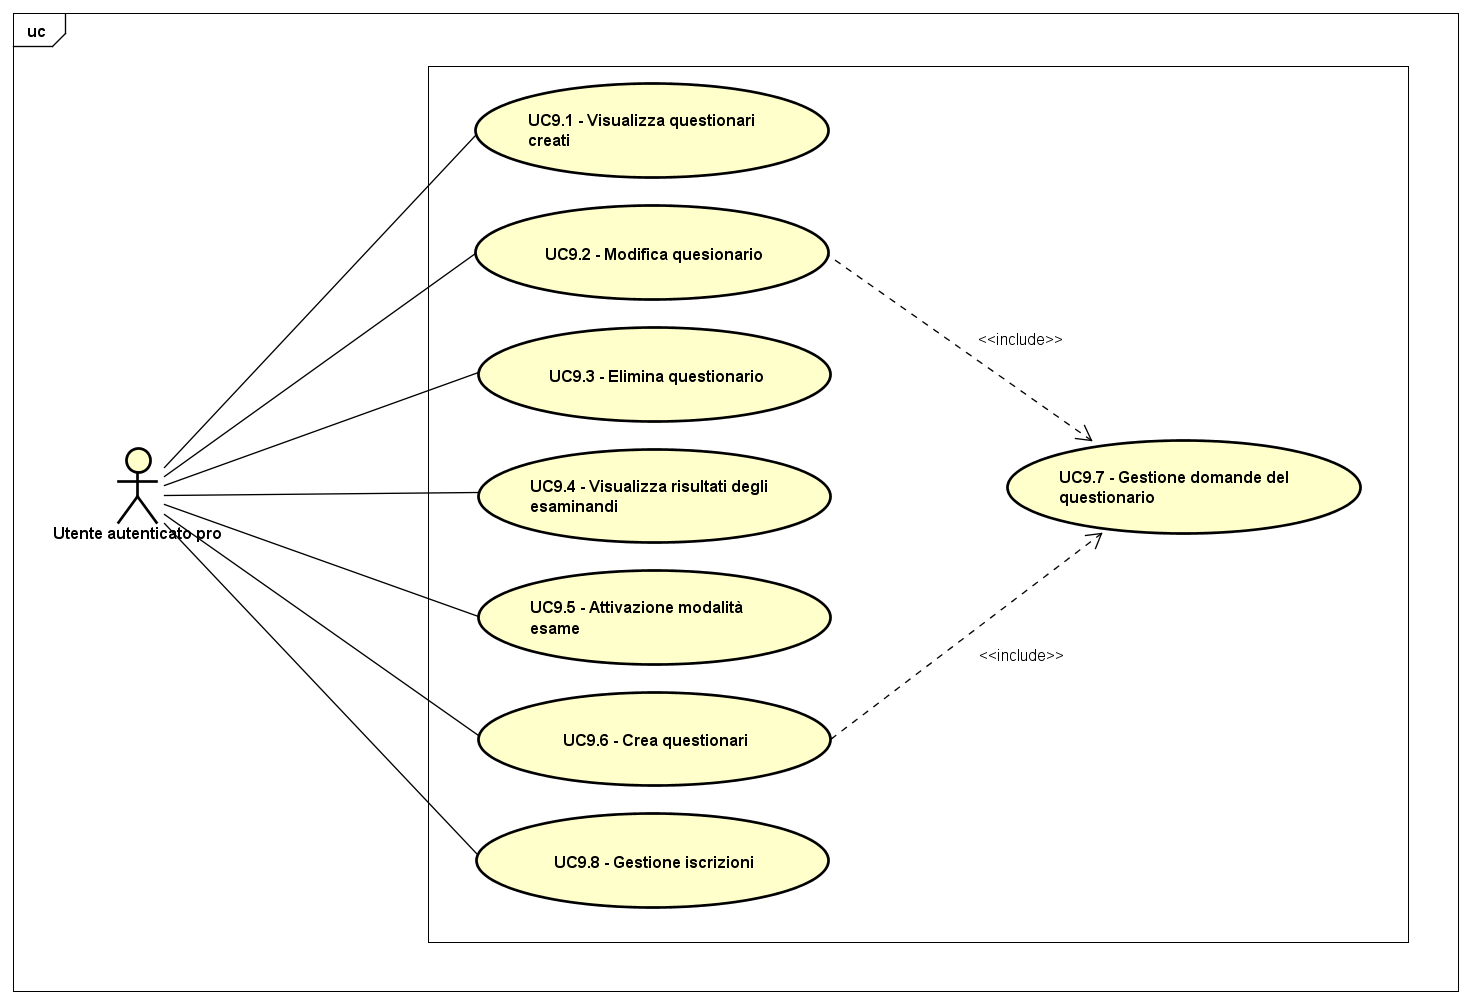
\includegraphics[scale=0.7,keepaspectratio]{UML/UC9.png}
			\caption{UC9.1.1: Visualizza questionari preferiti}
		\end{figure}
		\FloatBarrier
		\begin{itemize}
			\item \textbf{Attori}: 
			\item \textbf{Descrizione}: 
			\item \textbf{Precondizione}: 
			\item \textbf{Postcondizione}: 
			\item \textbf{Scenario principale}:
			\item \textbf{Inclusioni}:
			\item \textbf{Estensioni}:
			\item \textbf{Scenari alternativi}:
		\end{itemize}
		
		\paragraph{Caso d'uso UC9.1.2: Visualizza questionari creati}
		\label{UC9.1.2}
		\begin{figure}[h]
			\centering
		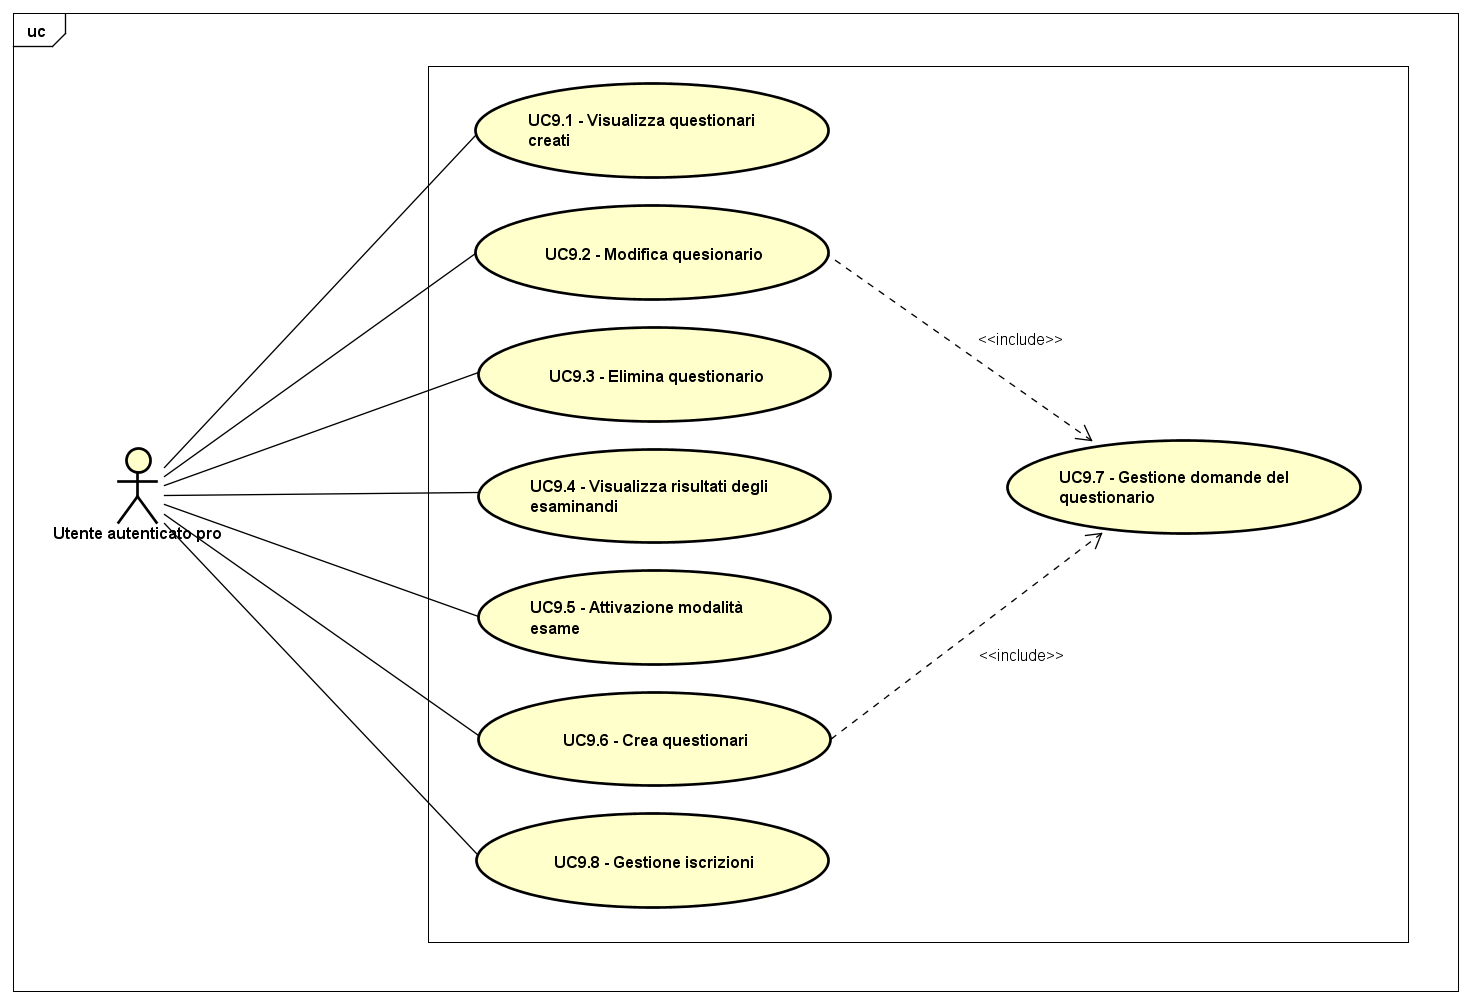
\includegraphics[scale=0.7,keepaspectratio]{UML/UC9.png}
			\caption{UC9.1.2: Visualizza questionari creati}
		\end{figure}
		\FloatBarrier
		\begin{itemize}
			\item \textbf{Attori}: 
			\item \textbf{Descrizione}: 
			\item \textbf{Precondizione}: 
			\item \textbf{Postcondizione}: 
			\item \textbf{Scenario principale}:
			\item \textbf{Inclusioni}:
			\item \textbf{Estensioni}:
			\item \textbf{Scenari alternativi}:
		\end{itemize}
		
			\subparagraph{Caso d'uso UC9.1.2.1: Modifica questionario}
			\label{UC9.1.2.1}
			\begin{figure}[h]
				\centering
			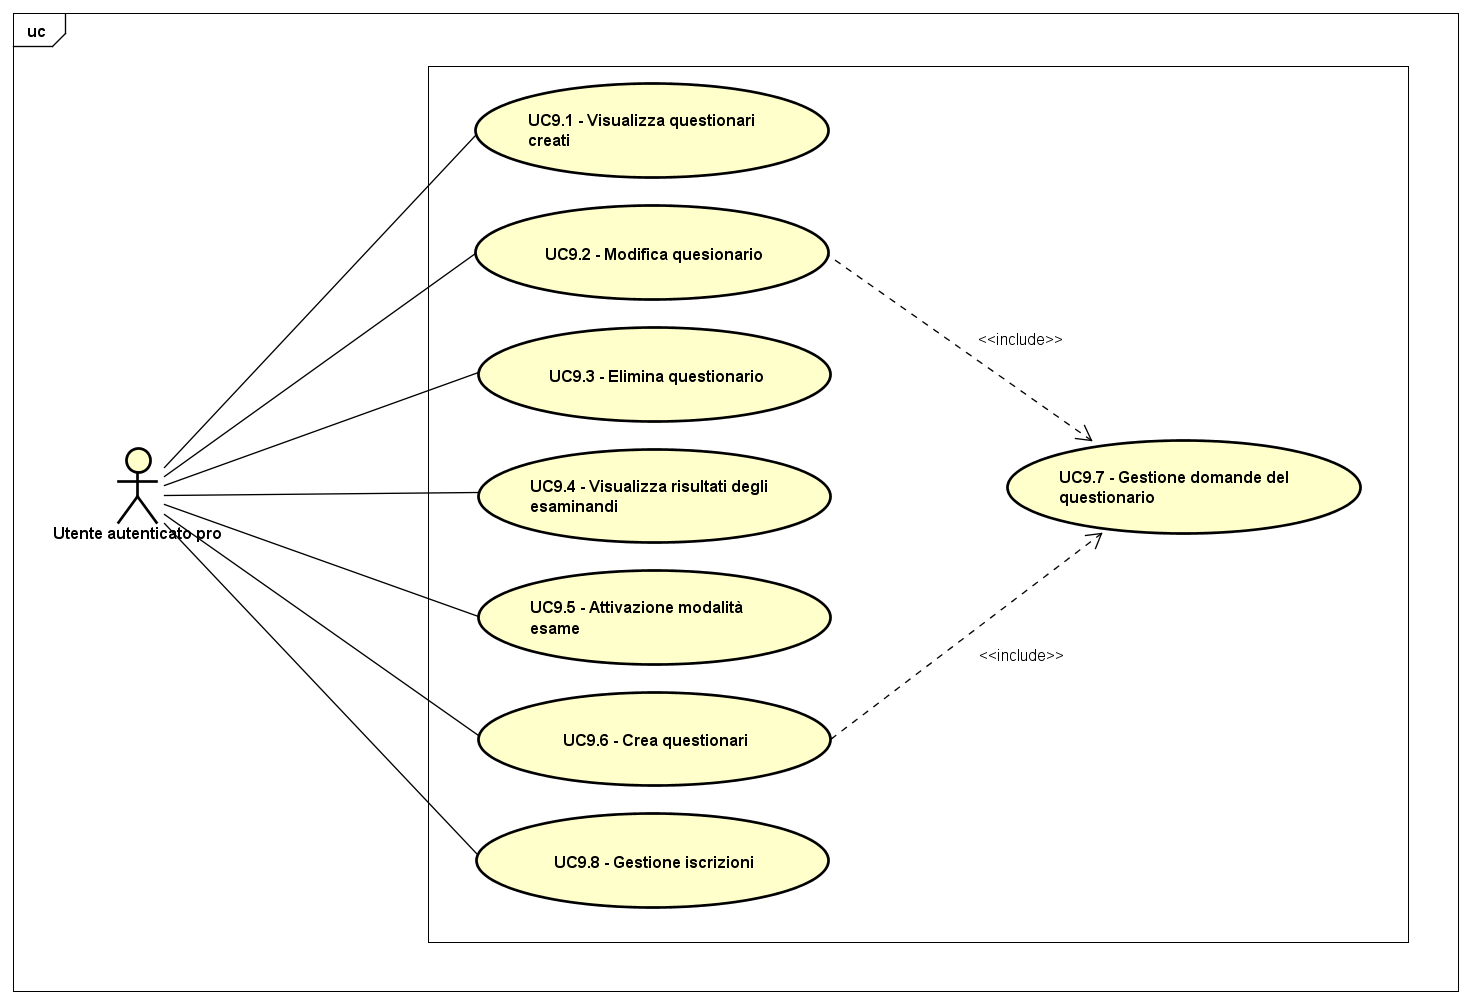
\includegraphics[scale=0.7,keepaspectratio]{UML/UC9.png}
				\caption{UC9.1.2.1: Modifica questionario}
			\end{figure}
			\FloatBarrier
			\begin{itemize}
				\item \textbf{Attori}: 
				\item \textbf{Descrizione}: 
				\item \textbf{Precondizione}: 
				\item \textbf{Postcondizione}: 
				\item \textbf{Scenario principale}:
				\item \textbf{Inclusioni}:
				\item \textbf{Estensioni}:
				\item \textbf{Scenari alternativi}:
			\end{itemize}
			
					\subsubparagraph{Caso d'uso UC9.1.2.1.1: Modifica tipologia questionario}
					\label{UC9.1.2.1.1}
					\begin{figure}[h]
						\centering
					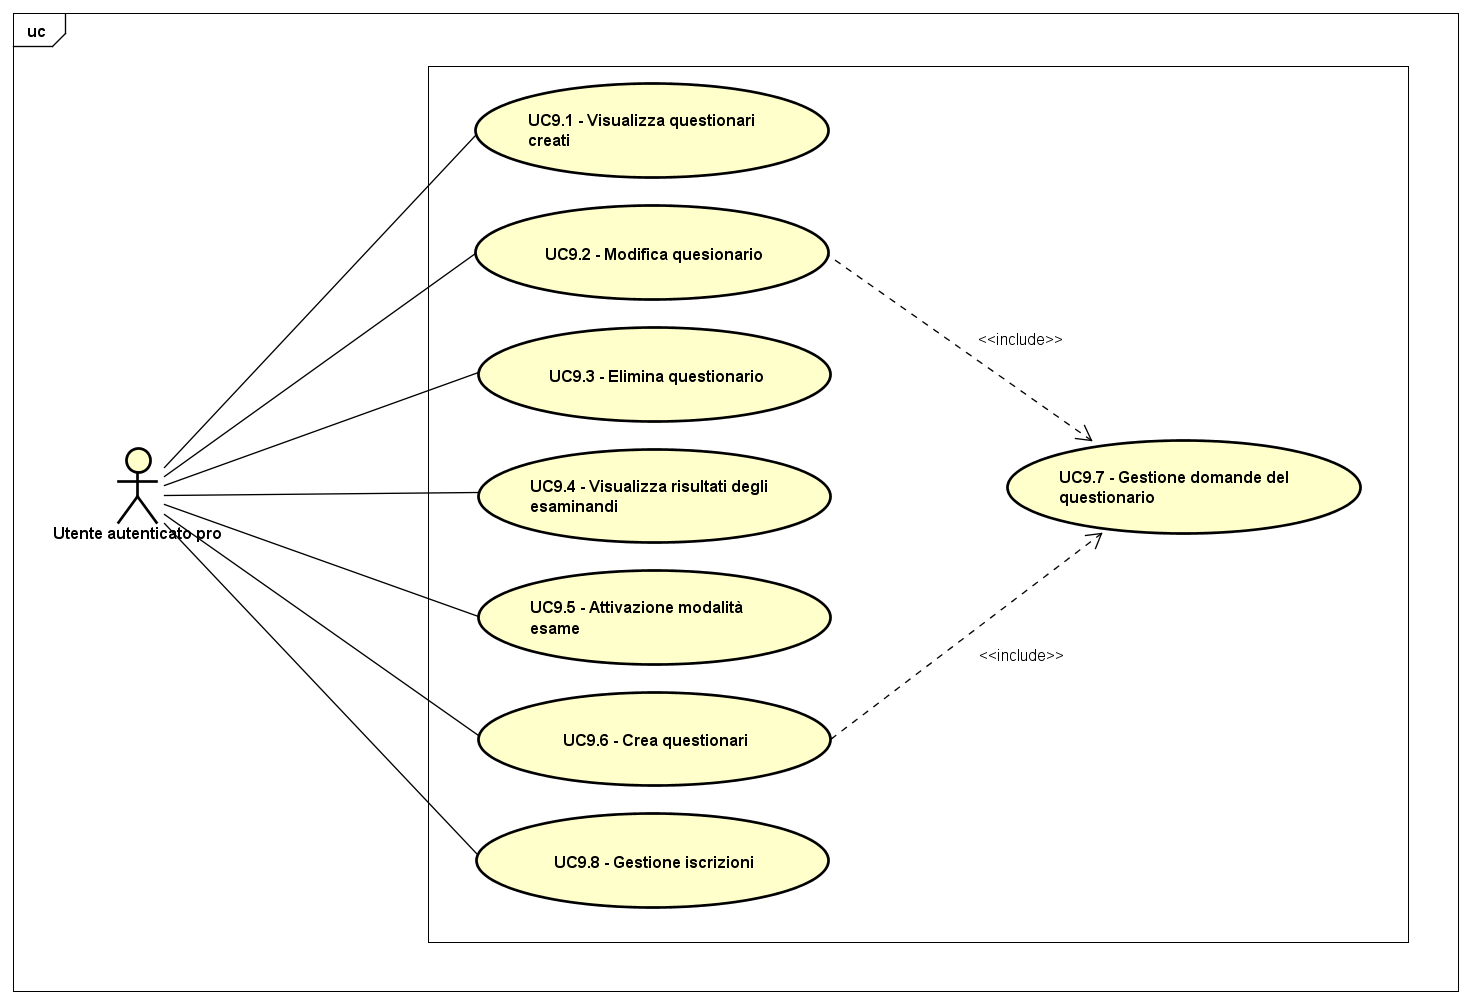
\includegraphics[scale=0.7,keepaspectratio]{UML/UC9.png}
						\caption{UC9.1.2.1.1: Modifica tipologia questionario}
					\end{figure}
					\FloatBarrier
					\begin{itemize}
						\item \textbf{Attori}: 
						\item \textbf{Descrizione}: 
						\item \textbf{Precondizione}: 
						\item \textbf{Postcondizione}: 
						\item \textbf{Scenario principale}:
						\item \textbf{Inclusioni}:
						\item \textbf{Estensioni}:
						\item \textbf{Scenari alternativi}:
					\end{itemize}
					
						\subsubsubparagraph{Caso d'uso UC9.1.2.1.1.1: Cambia tipologia utente}
						\label{UC9.1.2.1.1.1}
						\begin{figure}[h]
							\centering
						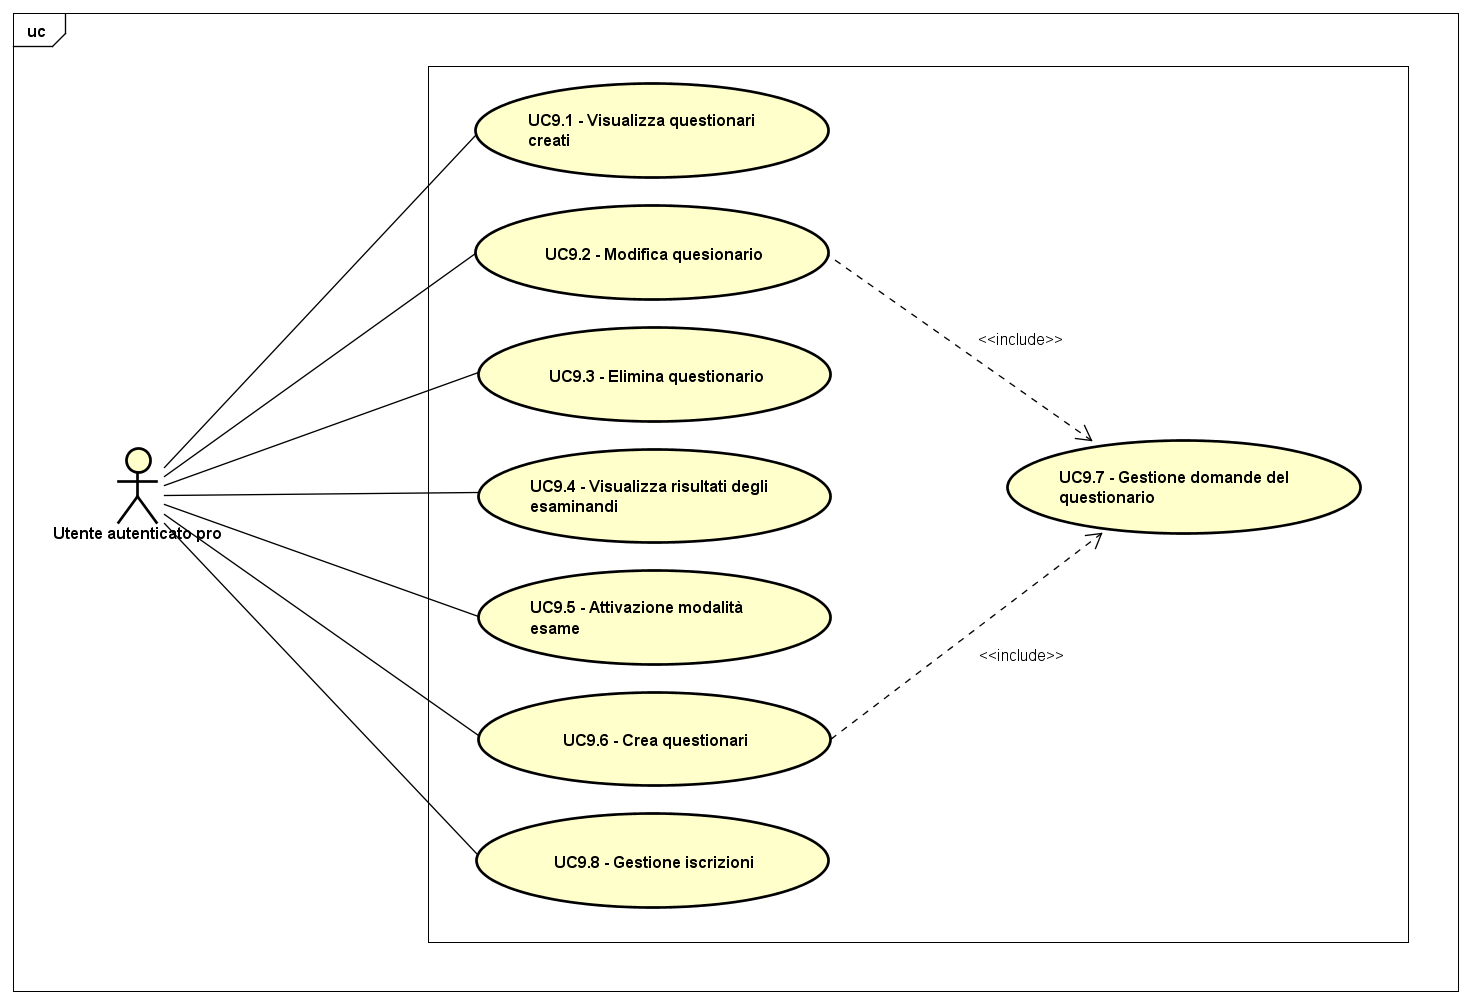
\includegraphics[scale=0.7,keepaspectratio]{UML/UC9.png}
							\caption{UC9.1.2.1.1.1: Cambia tipologia utente}
						\end{figure}
						\FloatBarrier
						\begin{itemize}
							\item \textbf{Attori}: 
							\item \textbf{Descrizione}: 
							\item \textbf{Precondizione}: 
							\item \textbf{Postcondizione}: 
							\item \textbf{Scenario principale}:
							\item \textbf{Inclusioni}:
							\item \textbf{Estensioni}:
							\item \textbf{Scenari alternativi}:
						\end{itemize}
						
					\subsubparagraph{Caso d'uso UC9.1.2.1.2: Modifica nome questionario}
					\label{UC9.1.2.1.2}
					\begin{figure}[h]
						\centering
					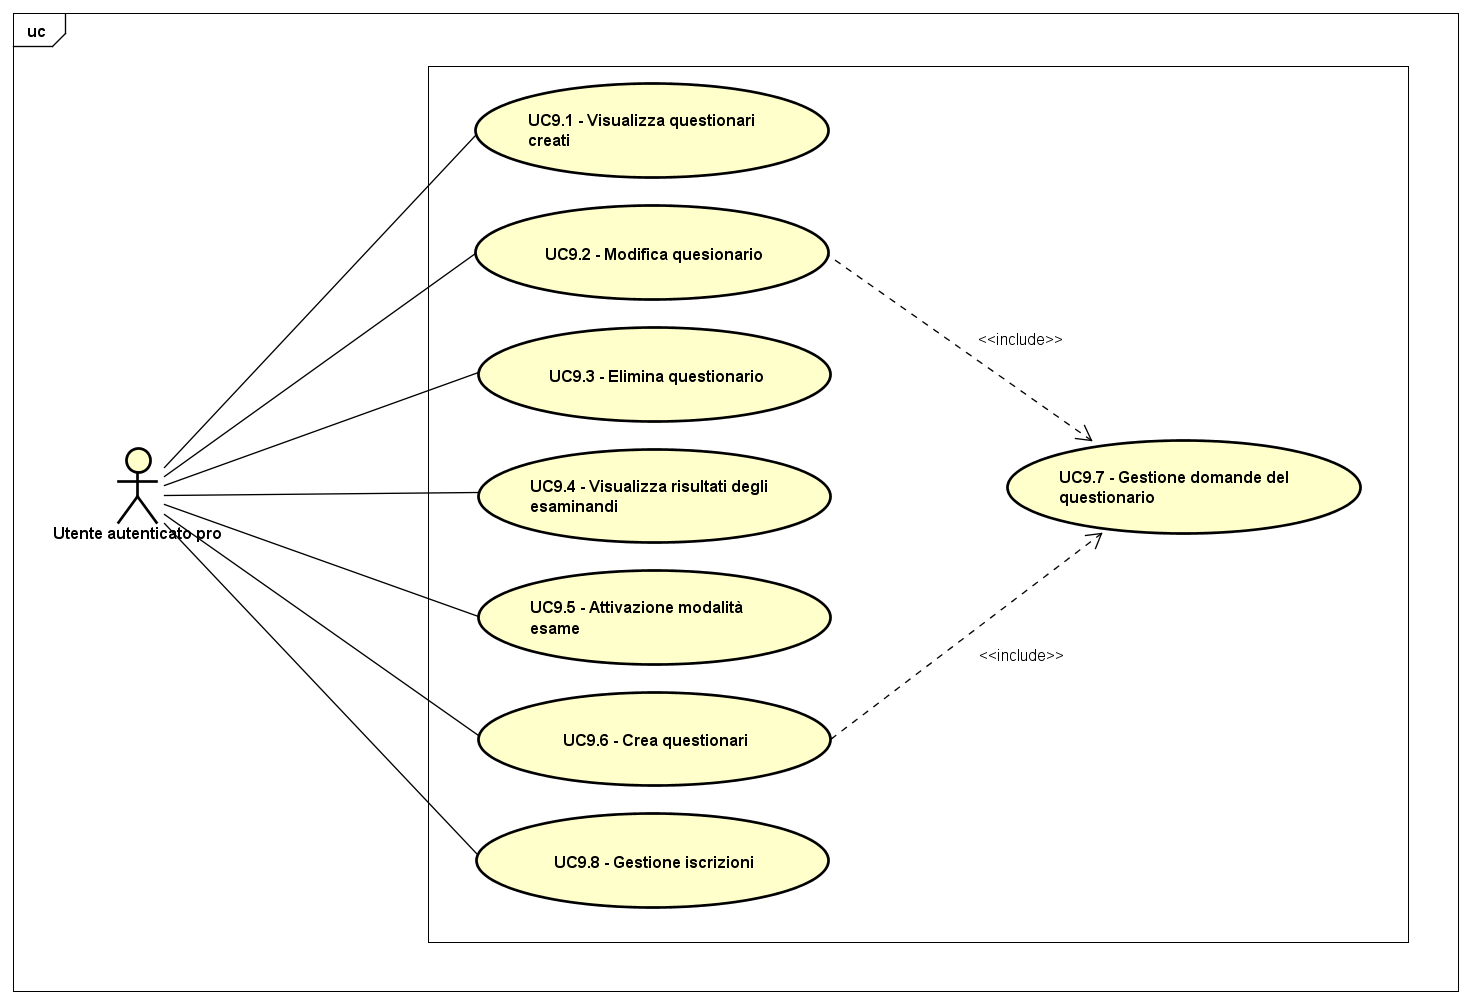
\includegraphics[scale=0.7,keepaspectratio]{UML/UC9.png}
						\caption{UC9.1.2.1.2: Modifica nome questionario}
					\end{figure}
					\FloatBarrier
					\begin{itemize}
						\item \textbf{Attori}: 
						\item \textbf{Descrizione}: 
						\item \textbf{Precondizione}: 
						\item \textbf{Postcondizione}: 
						\item \textbf{Scenario principale}:
						\item \textbf{Inclusioni}:
						\item \textbf{Estensioni}:
						\item \textbf{Scenari alternativi}:
					\end{itemize}
					
					\subsubparagraph{Caso d'uso UC9.1.2.1.3: Modifica categorie questionario}
					\label{UC9.1.2.1.3}
					\begin{figure}[h]
						\centering
					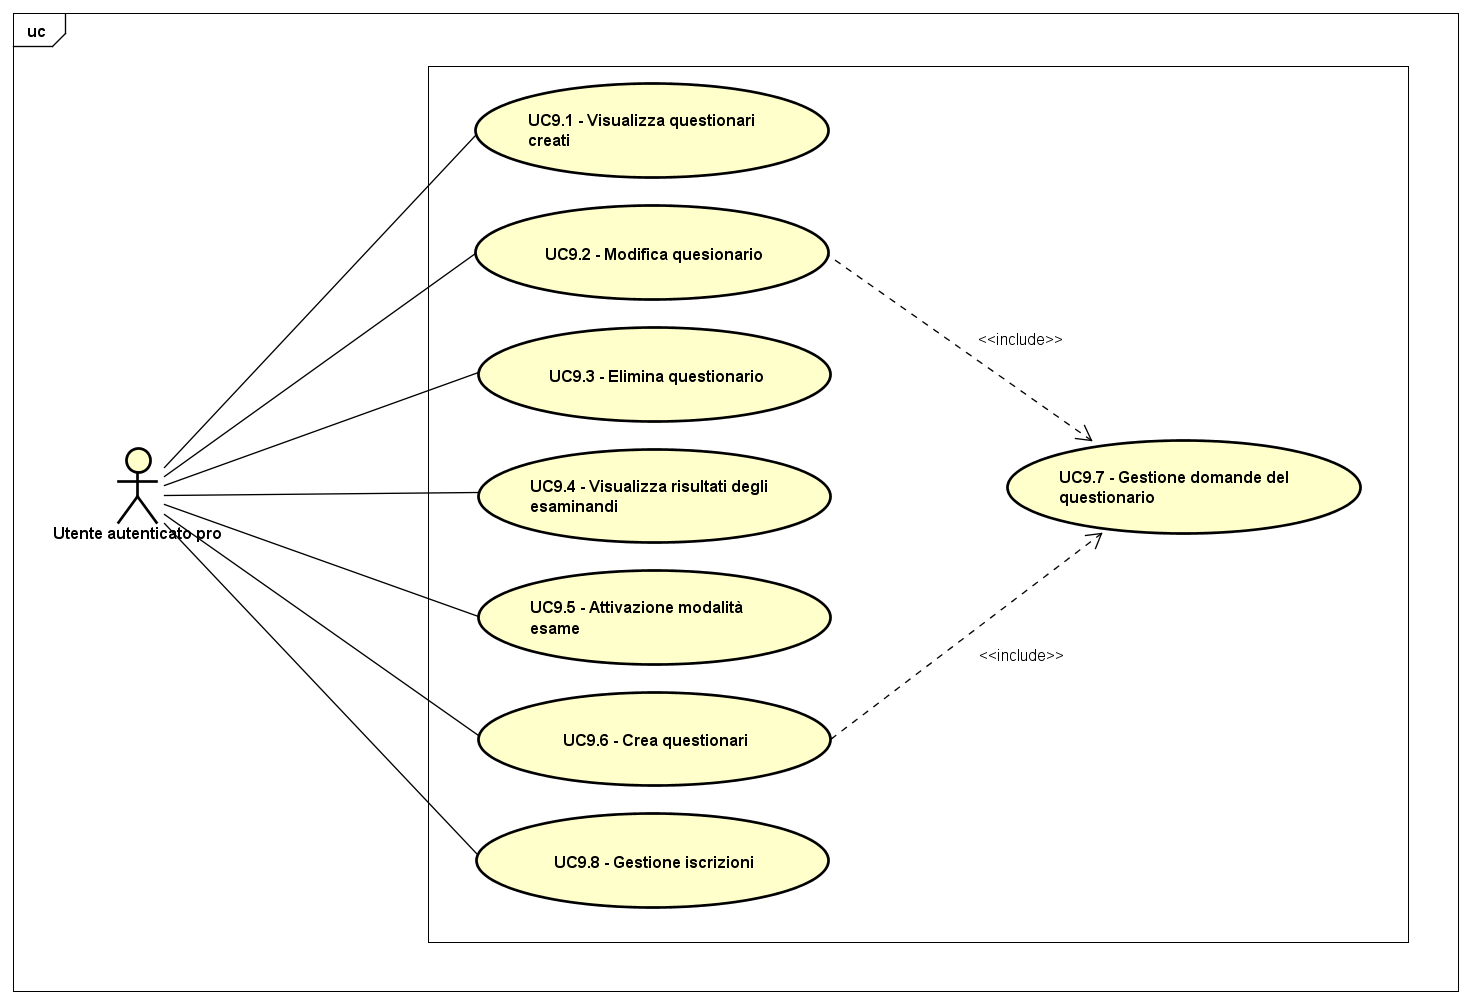
\includegraphics[scale=0.7,keepaspectratio]{UML/UC9.png}
						\caption{UC9.1.2.1.3: Modifica categorie questionario}
					\end{figure}
					\FloatBarrier
					\begin{itemize}
						\item \textbf{Attori}: 
						\item \textbf{Descrizione}: 
						\item \textbf{Precondizione}: 
						\item \textbf{Postcondizione}: 
						\item \textbf{Scenario principale}:
						\item \textbf{Inclusioni}:
						\item \textbf{Estensioni}:
						\item \textbf{Scenari alternativi}:
					\end{itemize}
					
						\subsubsubparagraph{Caso d'uso UC9.1.2.1.3.1: Crea categoria}
						\label{UC9.1.2.1.3.1}
						\begin{figure}[h]
							\centering
						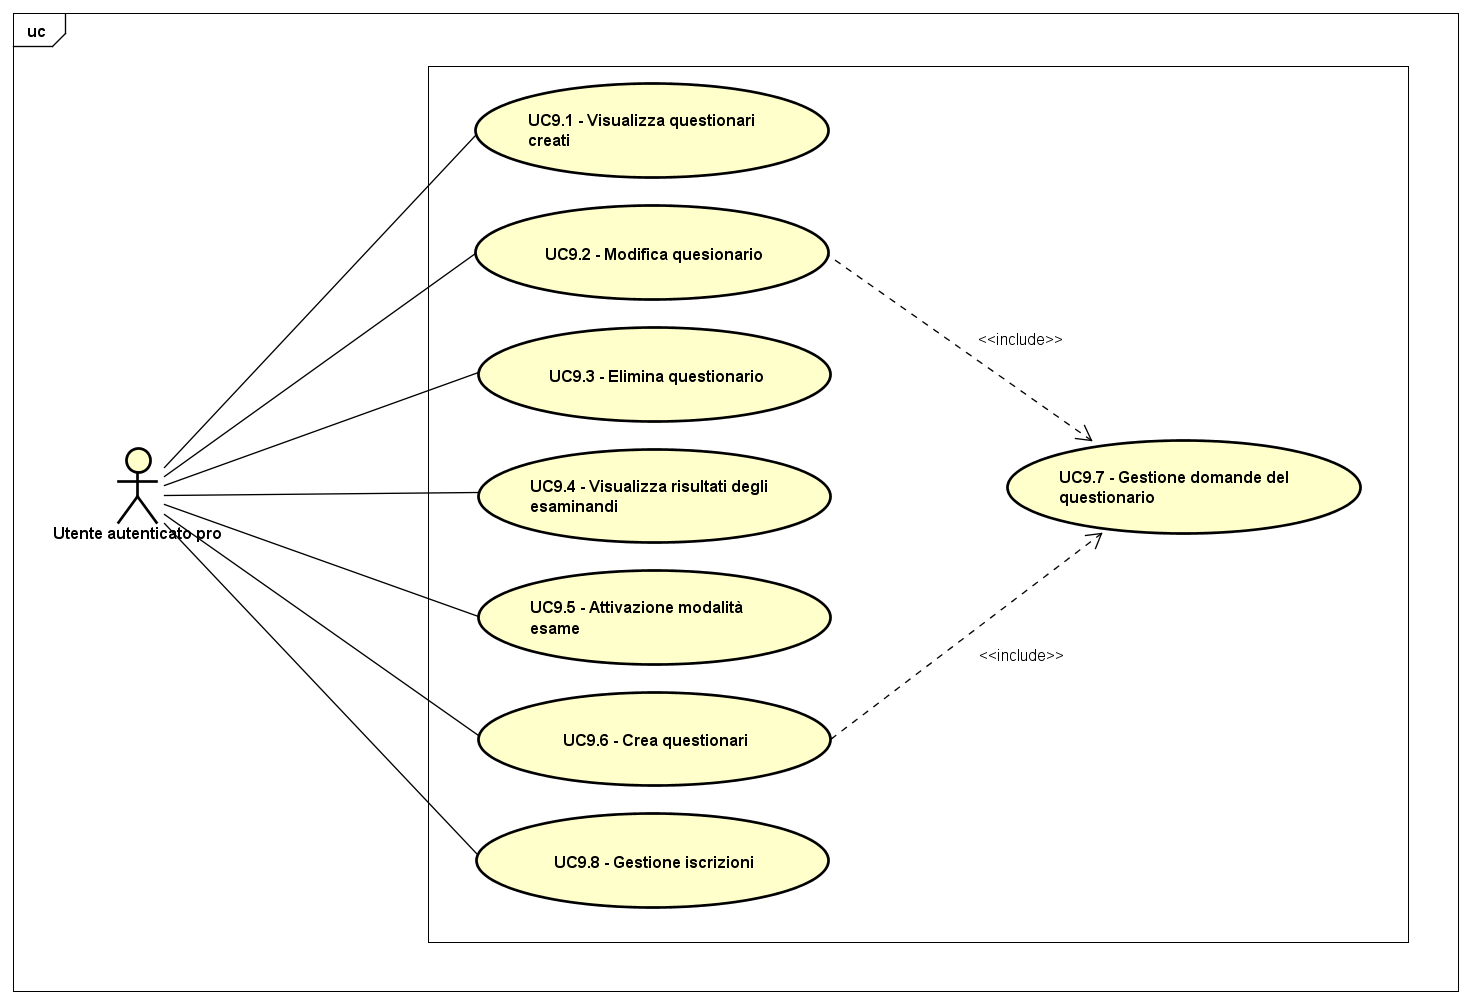
\includegraphics[scale=0.7,keepaspectratio]{UML/UC9.png}
							\caption{UC9.1.2.1.3.1: Crea categoria}
						\end{figure}
						\FloatBarrier
						\begin{itemize}
							\item \textbf{Attori}: 
							\item \textbf{Descrizione}: 
							\item \textbf{Precondizione}: 
							\item \textbf{Postcondizione}: 
							\item \textbf{Scenario principale}:
							\item \textbf{Inclusioni}:
							\item \textbf{Estensioni}:
							\item \textbf{Scenari alternativi}:
						\end{itemize}
						
					\subsubparagraph{Caso d'uso UC9.1.2.1.4: Gestione domande}
					\label{UC9.1.2.1.4}
					\begin{figure}[h]
						\centering
					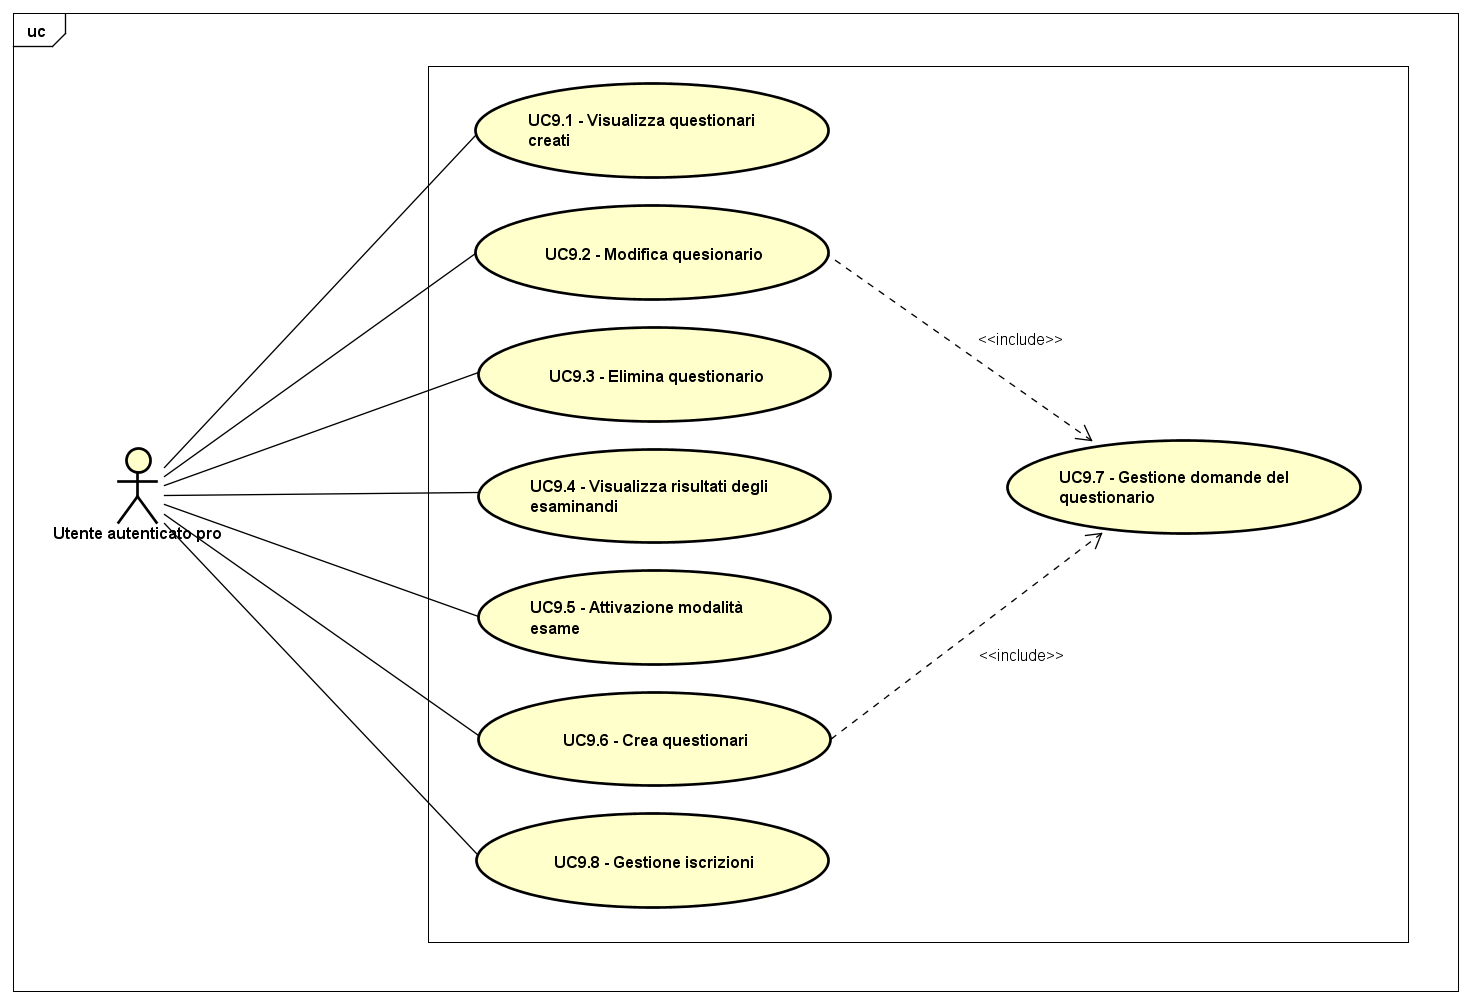
\includegraphics[scale=0.7,keepaspectratio]{UML/UC9.png}
						\caption{UC9.1.2.1.4: Gestione domande}
					\end{figure}
					\FloatBarrier
					\begin{itemize}
						\item \textbf{Attori}: 
						\item \textbf{Descrizione}: 
						\item \textbf{Precondizione}: 
						\item \textbf{Postcondizione}: 
						\item \textbf{Scenario principale}:
						\item \textbf{Inclusioni}:
						\item \textbf{Estensioni}:
						\item \textbf{Scenari alternativi}:
					\end{itemize}
					
						\subsubsubparagraph{Caso d'uso UC9.1.2.1.4.1: Seleziona altre domande}
						\label{UC9.1.2.1.4.1}
						\begin{figure}[h]
							\centering
						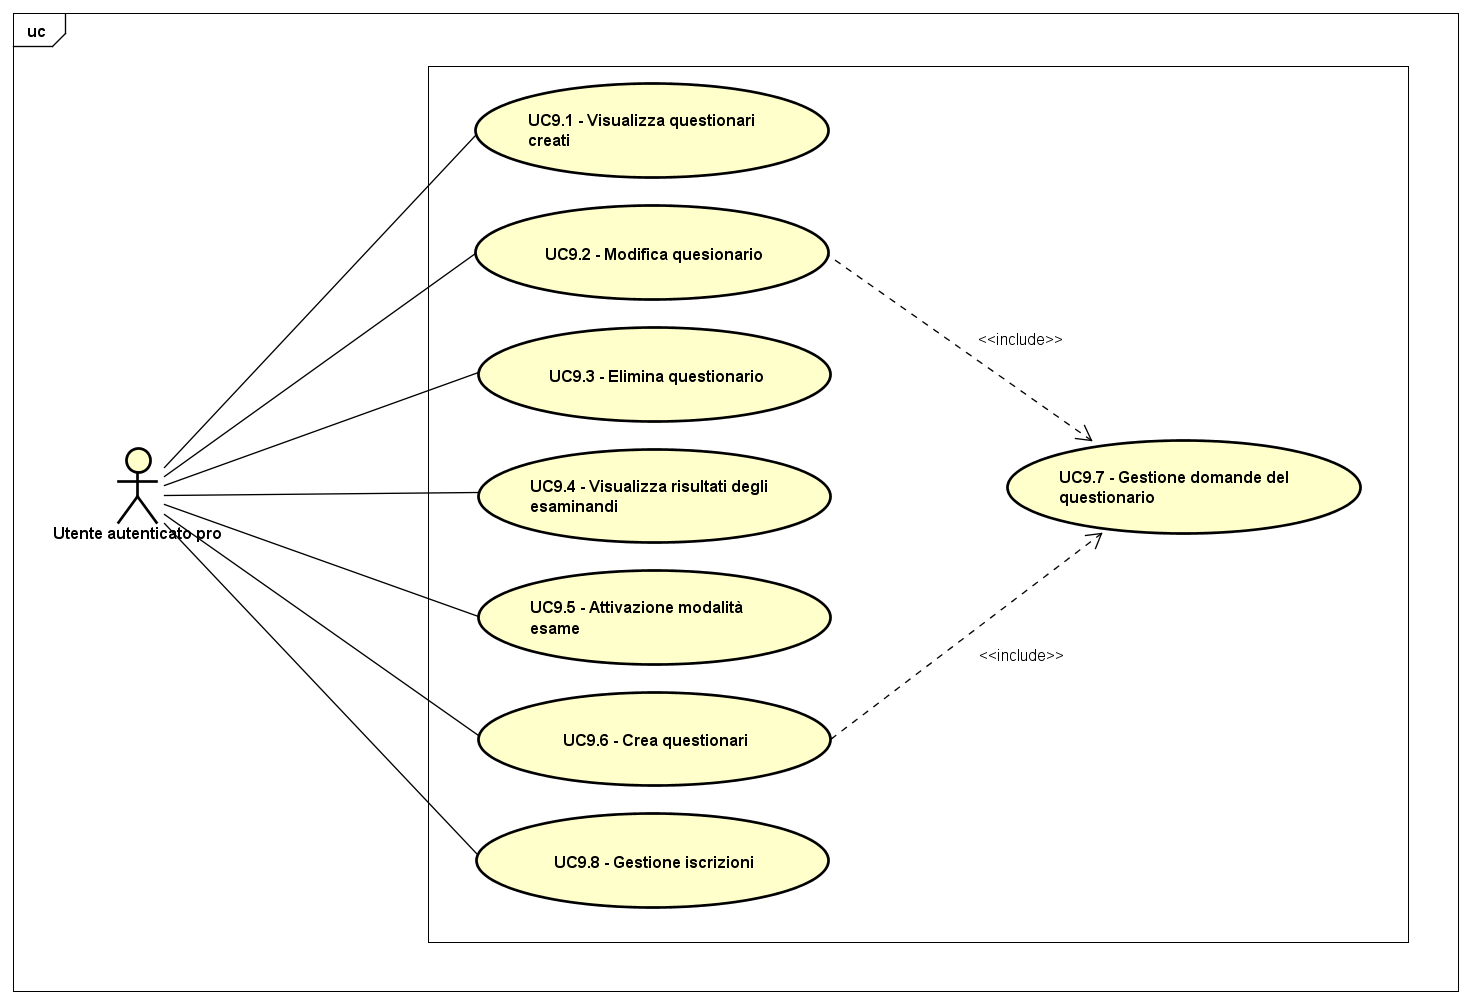
\includegraphics[scale=0.7,keepaspectratio]{UML/UC9.png}
							\caption{UC9.1.2.1.4.1: Seleziona altre domande}
						\end{figure}
						\FloatBarrier
						\begin{itemize}
							\item \textbf{Attori}: 
							\item \textbf{Descrizione}: 
							\item \textbf{Precondizione}: 
							\item \textbf{Postcondizione}: 
							\item \textbf{Scenario principale}:
							\item \textbf{Inclusioni}:
							\item \textbf{Estensioni}:
							\item \textbf{Scenari alternativi}:
						\end{itemize}
							
						\subsubsubparagraph{Caso d'uso UC9.1.2.1.4.2: Elimina domande}
						\label{UC9.1.2.1.4.2}
						\begin{figure}[h]
							\centering
						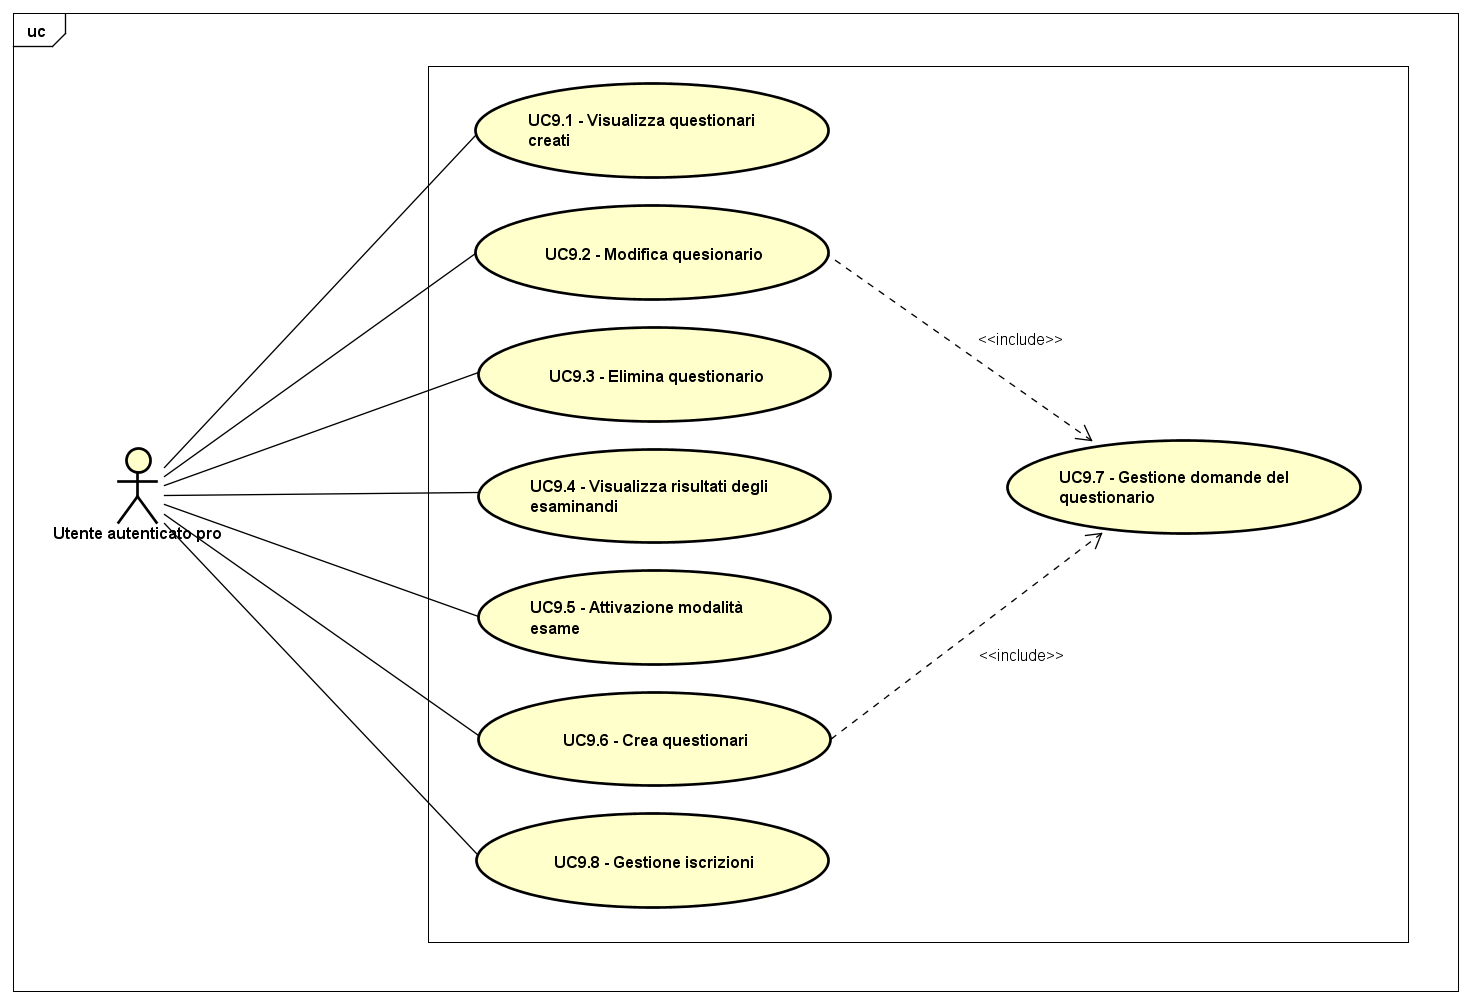
\includegraphics[scale=0.7,keepaspectratio]{UML/UC9.png}
							\caption{UC9.1.2.1.4.2: Elimina domande}
						\end{figure}
						\FloatBarrier
						\begin{itemize}
							\item \textbf{Attori}: 
							\item \textbf{Descrizione}: 
							\item \textbf{Precondizione}: 
							\item \textbf{Postcondizione}: 
							\item \textbf{Scenario principale}:
							\item \textbf{Inclusioni}:
							\item \textbf{Estensioni}:
							\item \textbf{Scenari alternativi}:
						\end{itemize}
						
						\subsubsubparagraph{Caso d'uso UC9.1.2.1.4.3: Crea domanda}
						\label{UC9.1.2.1.4.3}
						\begin{figure}[h]
							\centering
						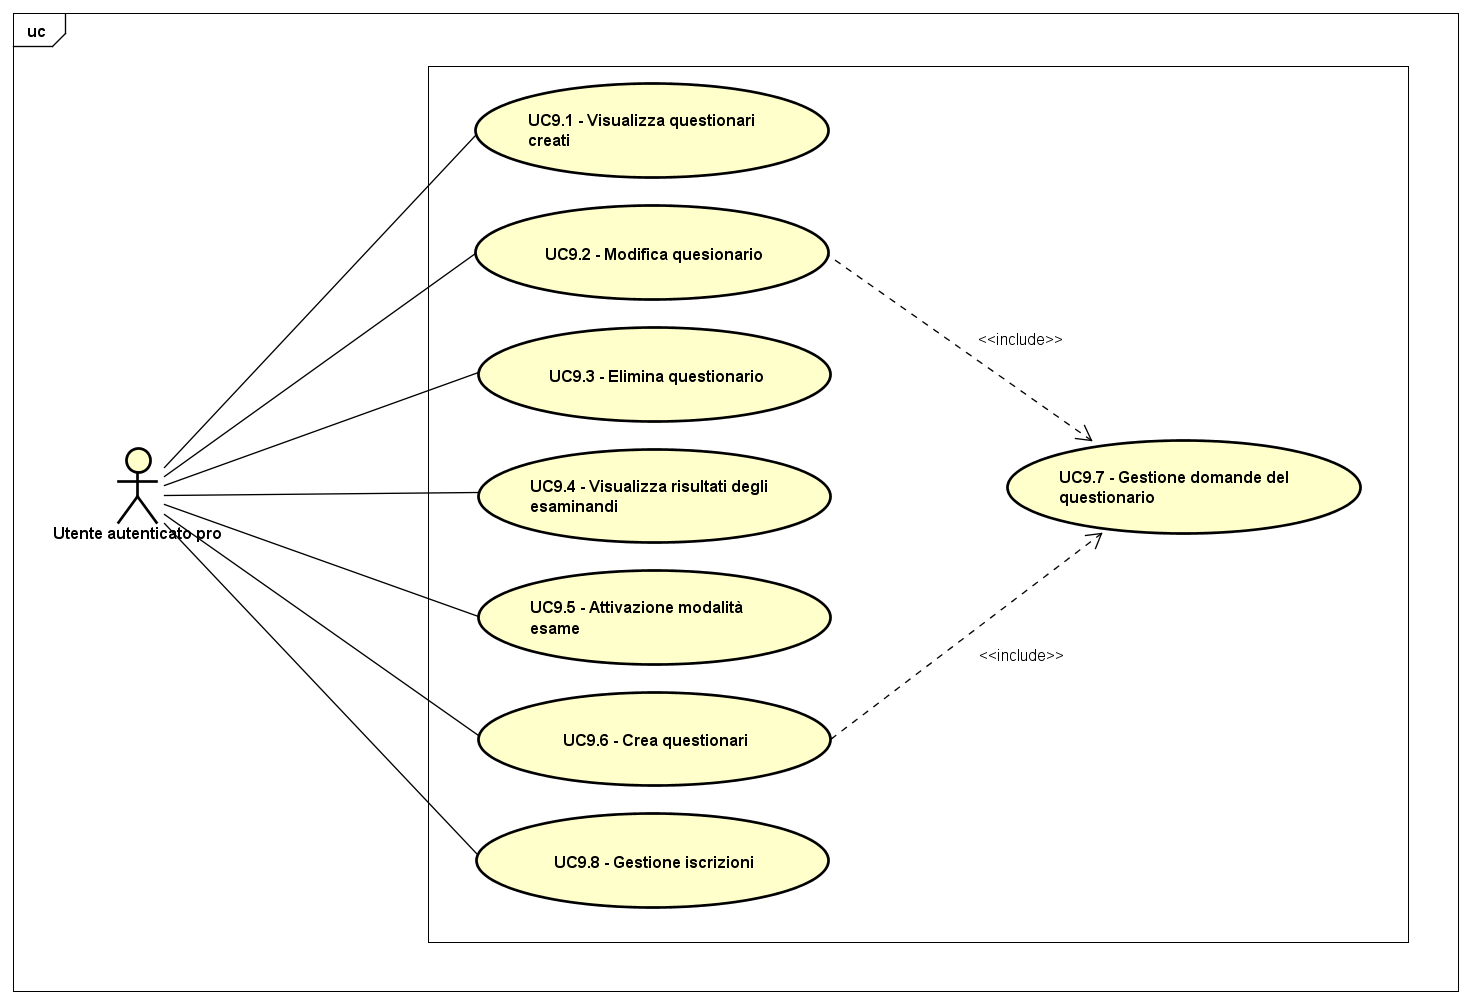
\includegraphics[scale=0.7,keepaspectratio]{UML/UC9.png}
							\caption{UC9.1.2.1.4.3: Crea domanda}
						\end{figure}
						\FloatBarrier
						\begin{itemize}
							\item \textbf{Attori}: 
							\item \textbf{Descrizione}: 
							\item \textbf{Precondizione}: 
							\item \textbf{Postcondizione}: 
							\item \textbf{Scenario principale}:
							\item \textbf{Inclusioni}:
							\item \textbf{Estensioni}:
							\item \textbf{Scenari alternativi}:
						\end{itemize}
						
					\subsubparagraph{Caso d'uso UC9.1.2.1.5: Resoconto modifiche}
					\label{UC9.1.2.1.5}
					\begin{figure}[h]
						\centering
					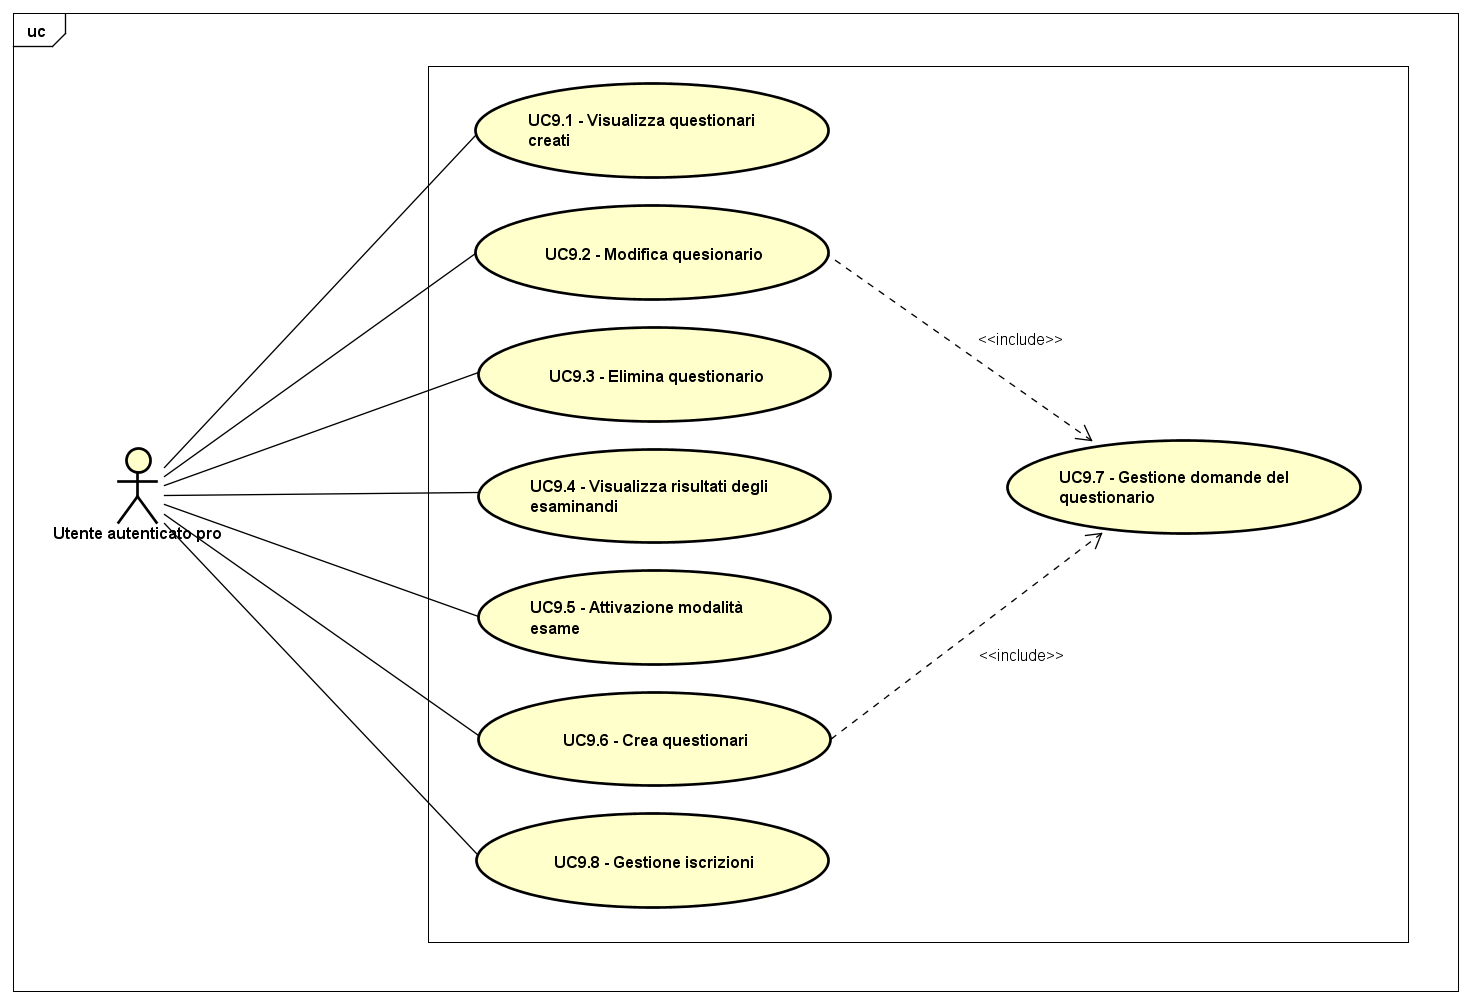
\includegraphics[scale=0.7,keepaspectratio]{UML/UC9.png}
						\caption{UC9.1.2.1.5: Resoconto modifiche}
					\end{figure}
					\FloatBarrier
					\begin{itemize}
						\item \textbf{Attori}: 
						\item \textbf{Descrizione}: 
						\item \textbf{Precondizione}: 
						\item \textbf{Postcondizione}: 
						\item \textbf{Scenario principale}:
						\item \textbf{Inclusioni}:
						\item \textbf{Estensioni}:
						\item \textbf{Scenari alternativi}:
					\end{itemize}
					
					\subsubparagraph{Caso d'uso UC9.1.2.1.6: Conferma modifiche}
					\label{UC9.1.2.1.6}
					\begin{figure}[h]
						\centering
					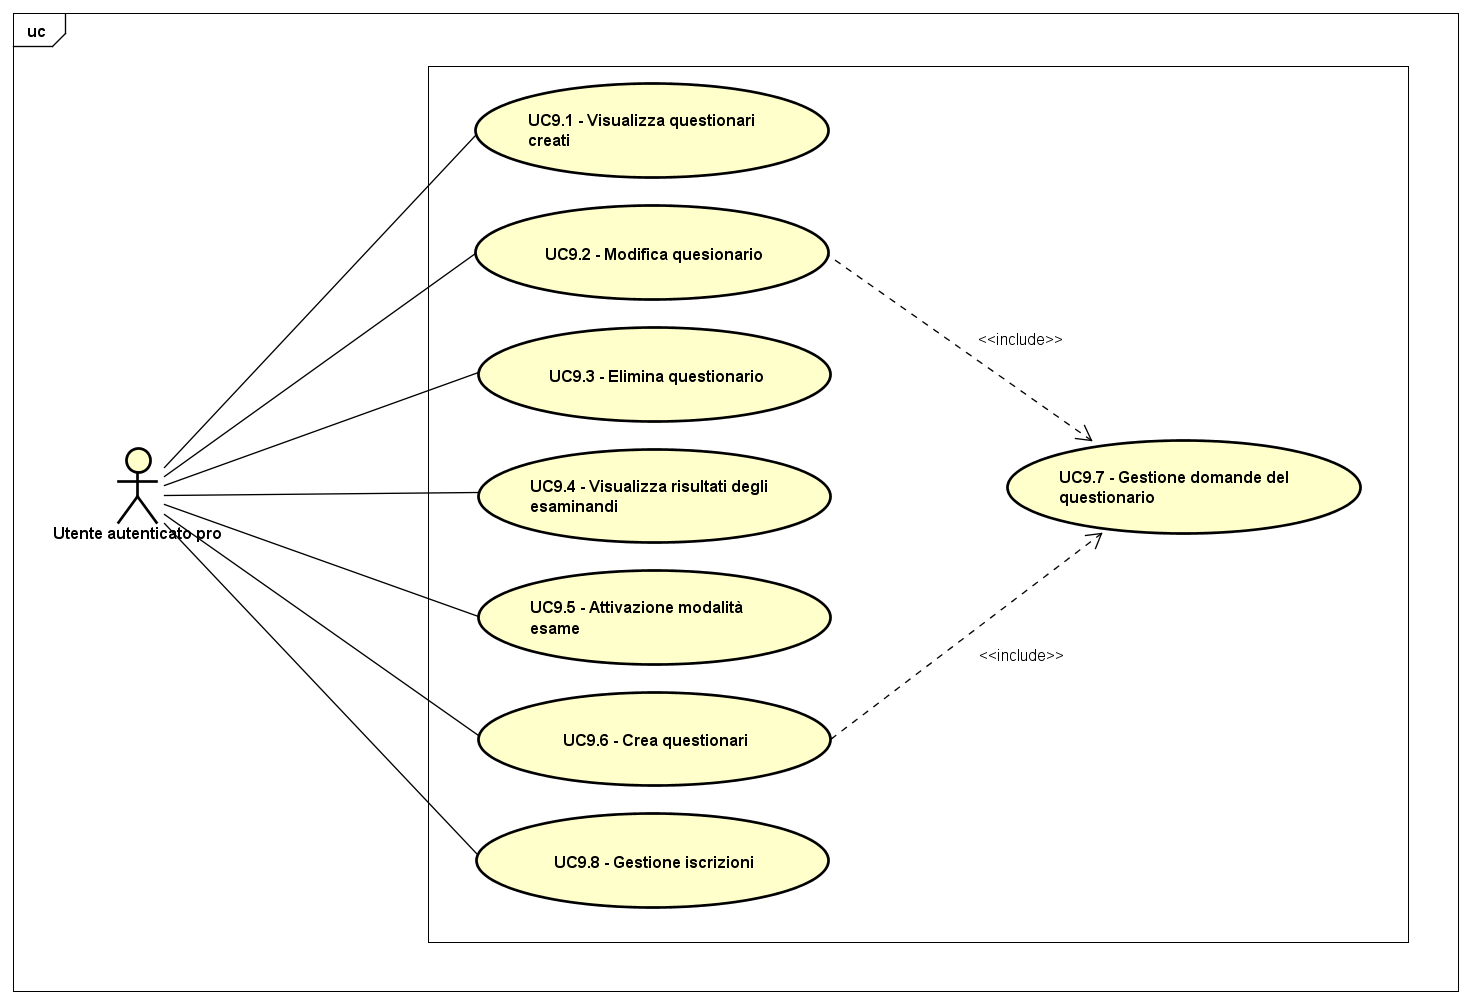
\includegraphics[scale=0.7,keepaspectratio]{UML/UC9.png}
						\caption{UC9.1.2.1.6: Conferma modifiche}
					\end{figure}
					\FloatBarrier
					\begin{itemize}
						\item \textbf{Attori}: 
						\item \textbf{Descrizione}: 
						\item \textbf{Precondizione}: 
						\item \textbf{Postcondizione}: 
						\item \textbf{Scenario principale}:
						\item \textbf{Inclusioni}:
						\item \textbf{Estensioni}:
						\item \textbf{Scenari alternativi}:
					\end{itemize}
					
					\subsubparagraph{Caso d'uso UC9.1.2.1.7: Annulla modifiche}
					\label{UC9.1.2.1.7}
					\begin{figure}[h]
						\centering
					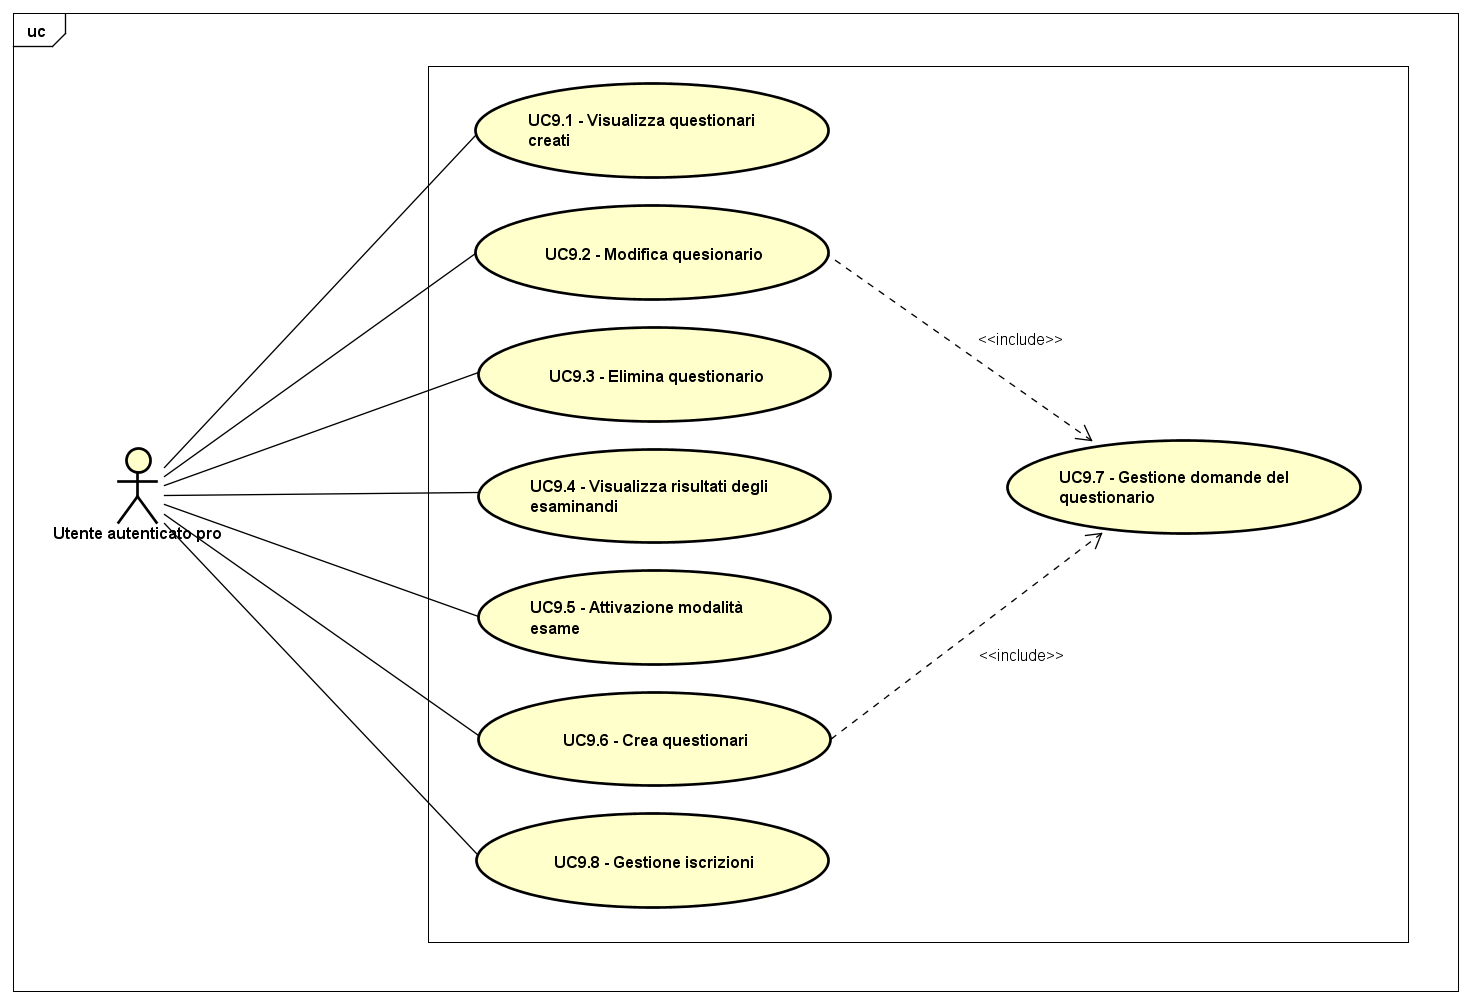
\includegraphics[scale=0.7,keepaspectratio]{UML/UC9.png}
						\caption{UC9.1.2.1.7: Annulla modifiche}
					\end{figure}
					\FloatBarrier
					\begin{itemize}
						\item \textbf{Attori}: 
						\item \textbf{Descrizione}: 
						\item \textbf{Precondizione}: 
						\item \textbf{Postcondizione}: 
						\item \textbf{Scenario principale}:
						\item \textbf{Inclusioni}:
						\item \textbf{Estensioni}:
						\item \textbf{Scenari alternativi}:
					\end{itemize}
					
			\subparagraph{Caso d'uso UC9.1.2.2: Elimina questionario}
			\label{UC9.1.2.2}
			\begin{figure}[h]
				\centering
			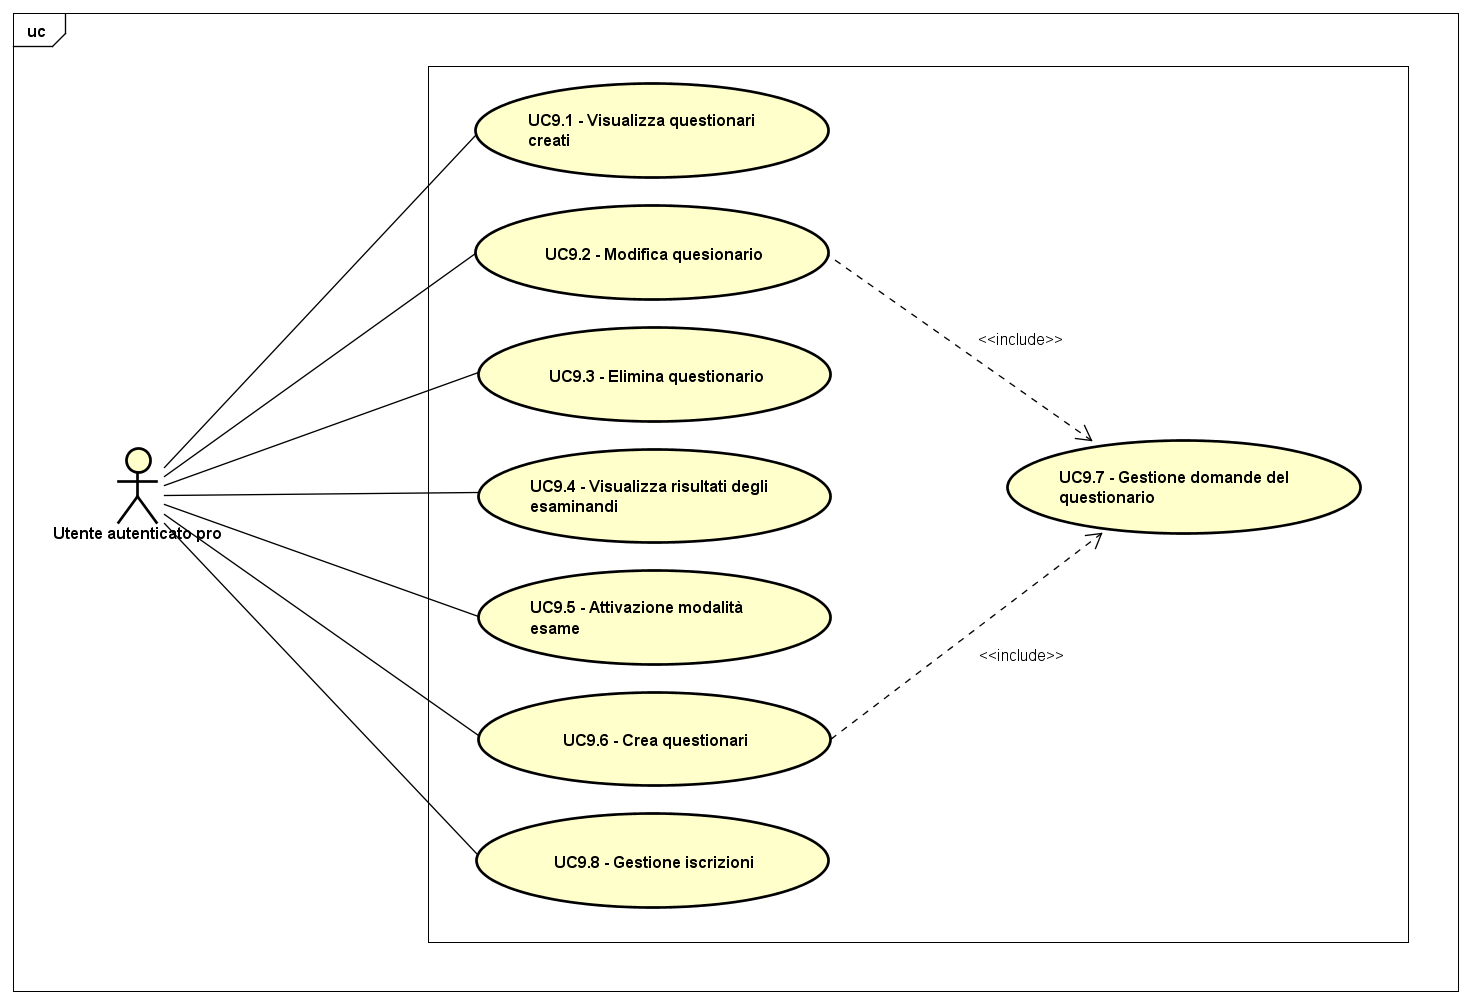
\includegraphics[scale=0.7,keepaspectratio]{UML/UC9.png}
				\caption{UC9.1.2.2: Elimina questionario}
			\end{figure}
			\FloatBarrier
			\begin{itemize}
				\item \textbf{Attori}: 
				\item \textbf{Descrizione}: 
				\item \textbf{Precondizione}: 
				\item \textbf{Postcondizione}: 
				\item \textbf{Scenario principale}:
				\item \textbf{Inclusioni}:
				\item \textbf{Estensioni}:
				\item \textbf{Scenari alternativi}:
			\end{itemize}
			
				\subsubparagraph{Caso d'uso UC9.1.2.2.1: Conferma eliminazione}
				\label{UC9.1.2.2.1}
				\begin{figure}[h]
					\centering
				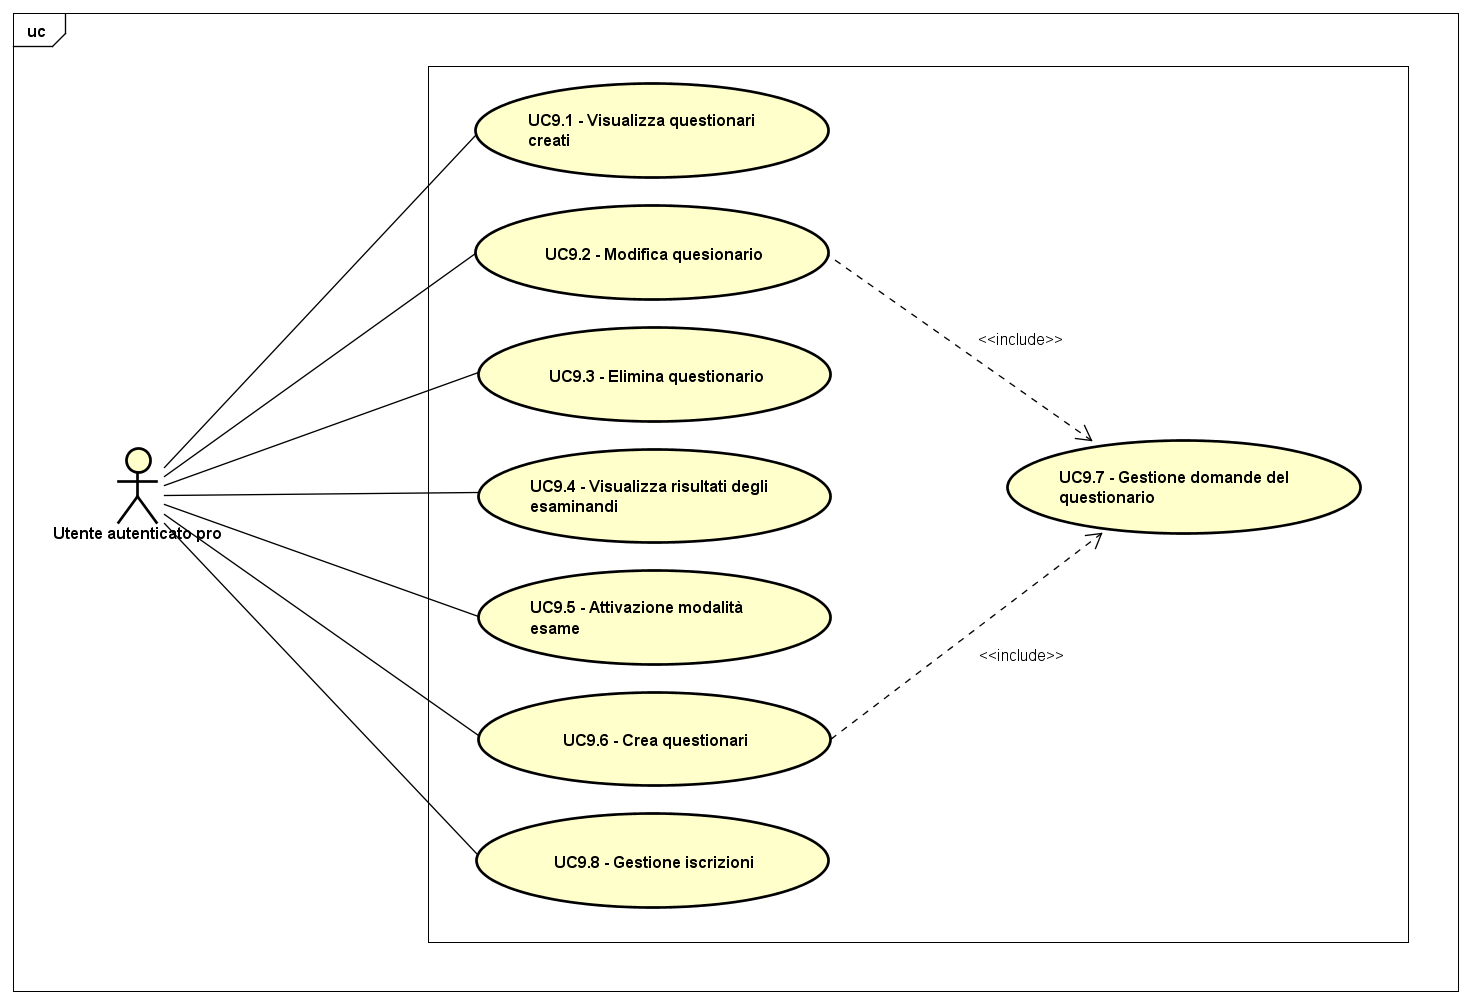
\includegraphics[scale=0.7,keepaspectratio]{UML/UC9.png}
					\caption{UC9.1.2.2.1: Conferma eliminazione}
				\end{figure}
				\FloatBarrier
				\begin{itemize}
					\item \textbf{Attori}: 
					\item \textbf{Descrizione}: 
					\item \textbf{Precondizione}: 
					\item \textbf{Postcondizione}: 
					\item \textbf{Scenario principale}:
					\item \textbf{Inclusioni}:
					\item \textbf{Estensioni}:
					\item \textbf{Scenari alternativi}:
				\end{itemize}
				
				\subsubparagraph{Caso d'uso UC9.1.2.2.2: Annulla eliminazione}
				\label{UC9.1.2.2.2}
				\begin{figure}[h]
					\centering
				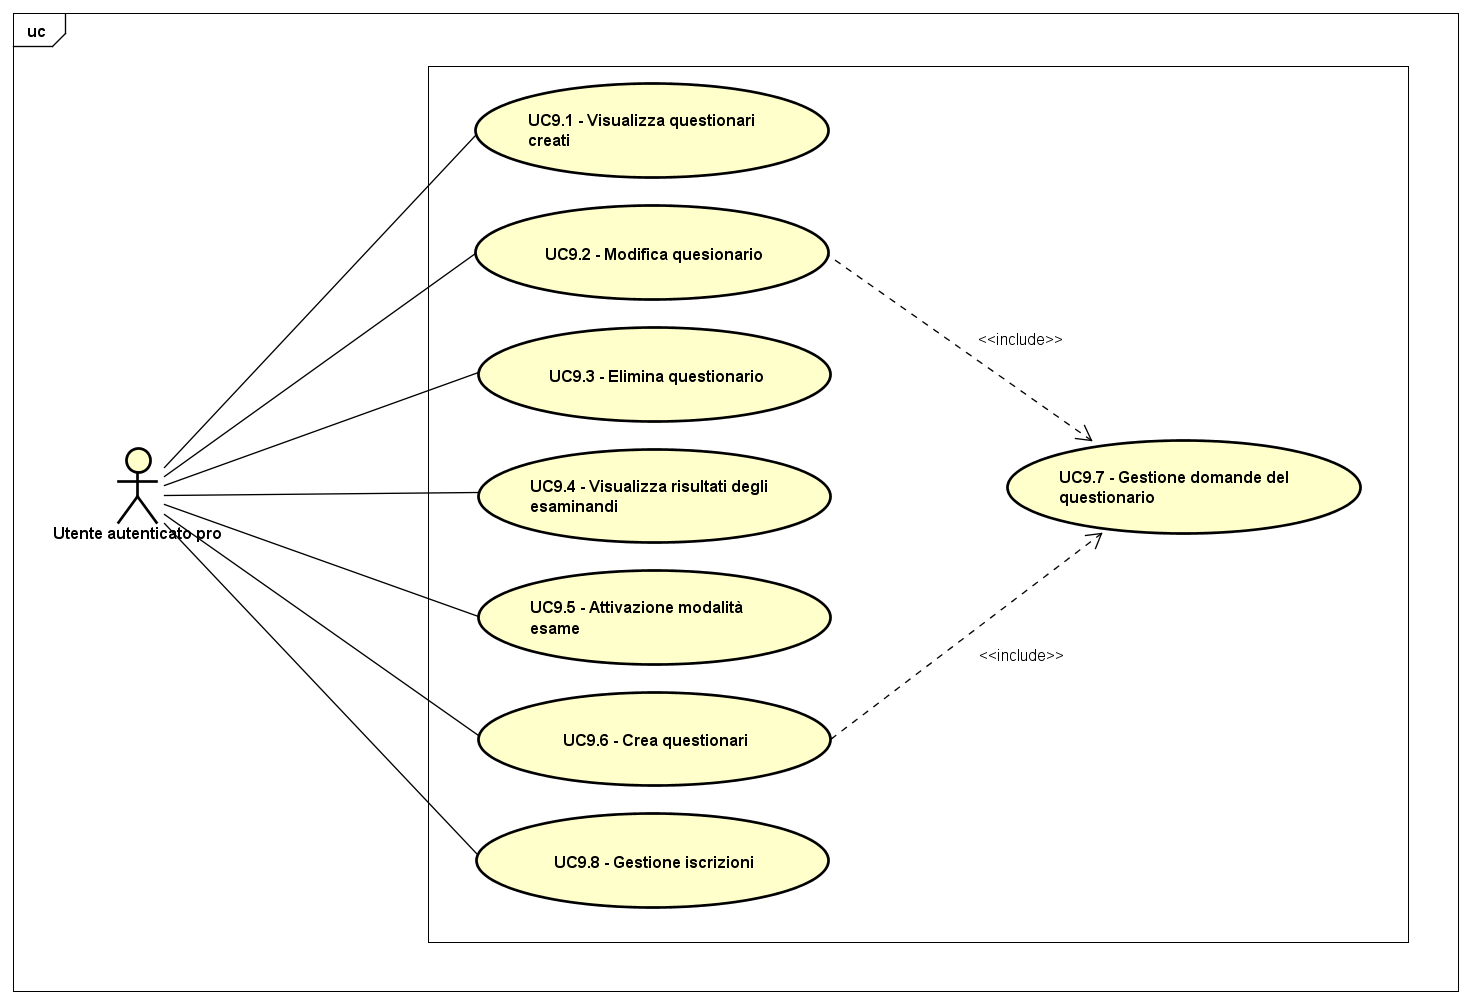
\includegraphics[scale=0.7,keepaspectratio]{UML/UC9.png}
					\caption{UC9.1.2.2.2: Annulla eliminazione}
				\end{figure}
				\FloatBarrier
				\begin{itemize}
					\item \textbf{Attori}: 
					\item \textbf{Descrizione}: 
					\item \textbf{Precondizione}: 
					\item \textbf{Postcondizione}: 
					\item \textbf{Scenario principale}:
					\item \textbf{Inclusioni}:
					\item \textbf{Estensioni}:
					\item \textbf{Scenari alternativi}:
				\end{itemize}
				
	\subsubsection{Caso d'uso UC9.2: Crea questionari}
	\label{UC9.2}
	\begin{figure}[h]
		\centering
	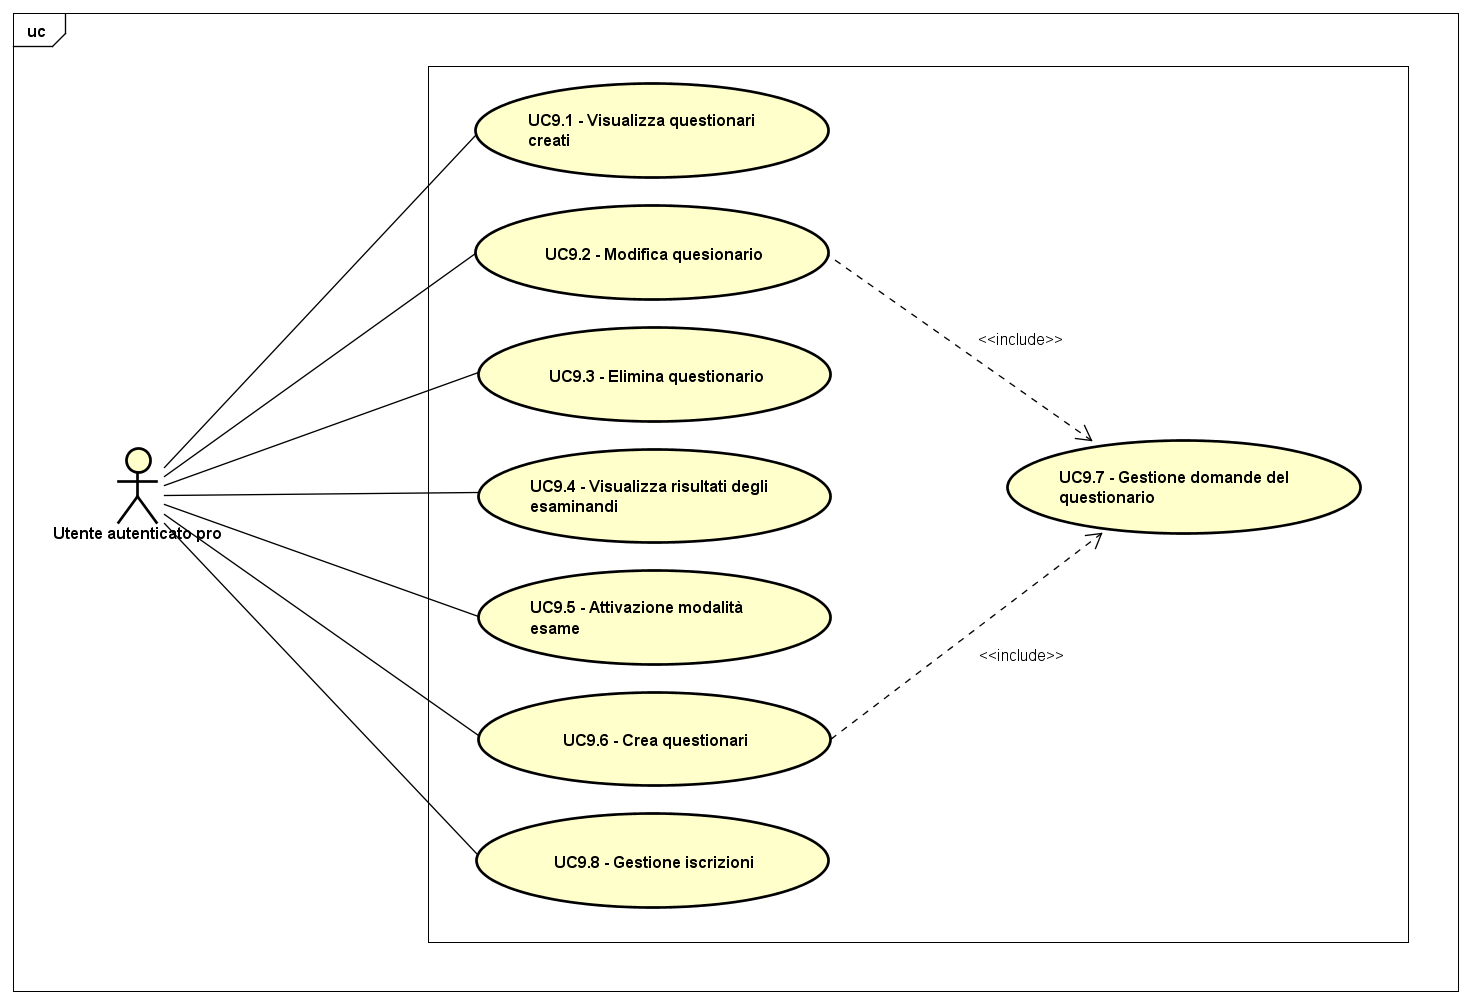
\includegraphics[scale=0.7,keepaspectratio]{UML/UC9.png}
		\caption{UC9.2: Crea questionari}
	\end{figure}
	\FloatBarrier
	\begin{itemize}
		\item \textbf{Attori}: 
		\item \textbf{Descrizione}: 
		\item \textbf{Precondizione}: 
		\item \textbf{Postcondizione}: 
		\item \textbf{Scenario principale}:
		\item \textbf{Inclusioni}:
		\item \textbf{Estensioni}:
		\item \textbf{Scenari alternativi}:
	\end{itemize}
	
		\paragraph{Caso d'uso UC9.2.1: Seleziona tipologia questionario}
		\label{UC9.2.1}
		\begin{figure}[h]
			\centering
		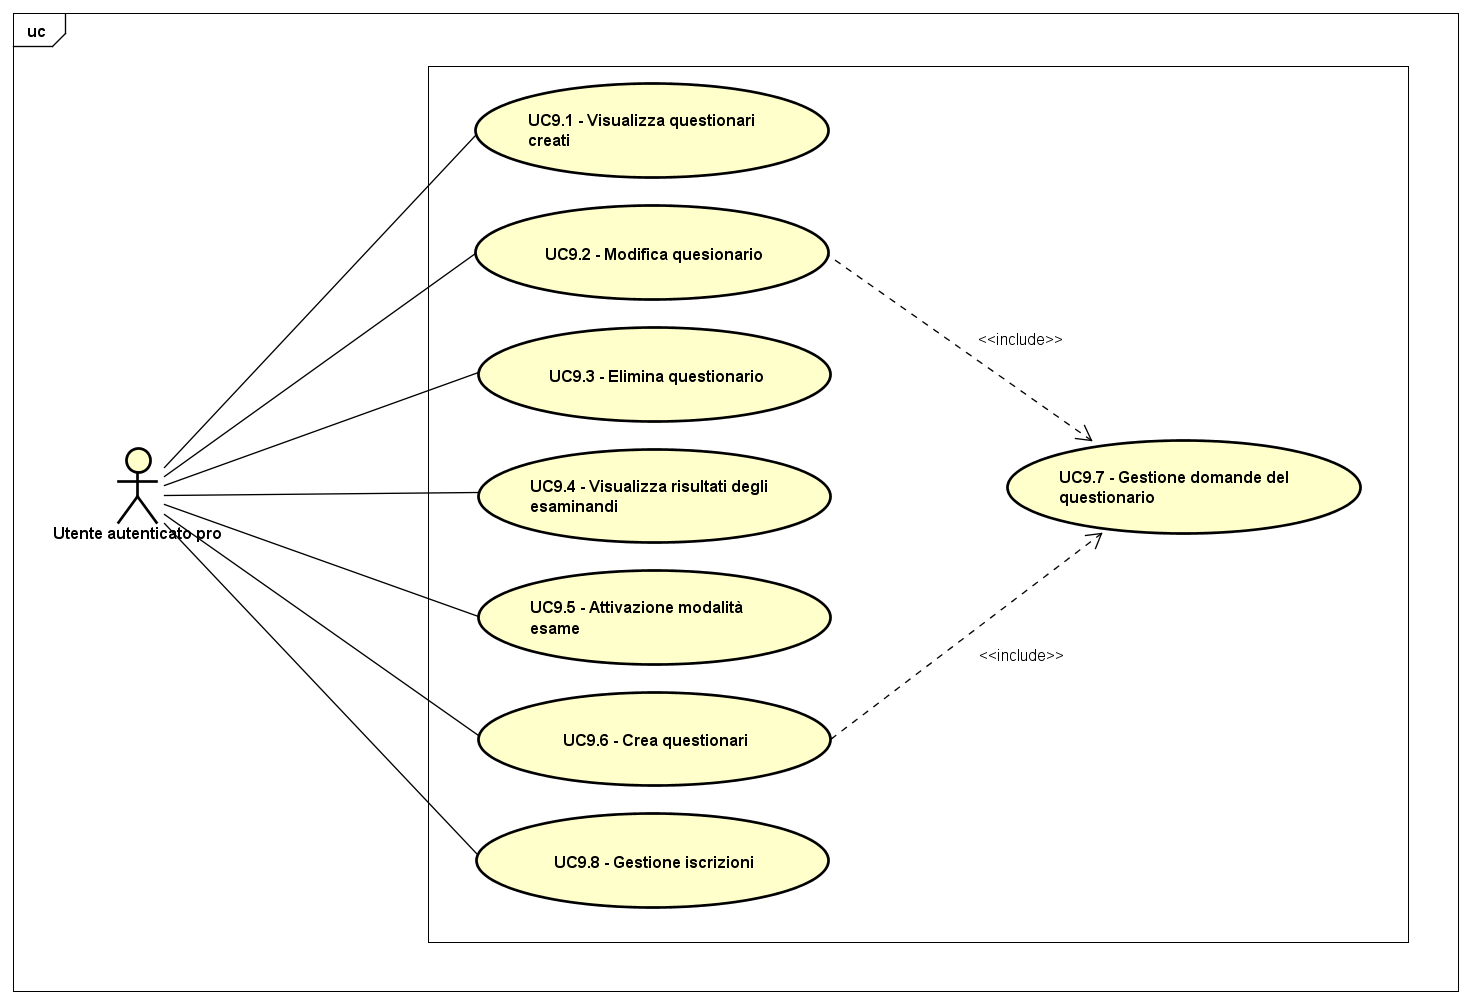
\includegraphics[scale=0.7,keepaspectratio]{UML/UC9.png}
			\caption{UC9.2.1: Seleziona tipologia questionario}
		\end{figure}
		\FloatBarrier
		\begin{itemize}
			\item \textbf{Attori}: 
			\item \textbf{Descrizione}: 
			\item \textbf{Precondizione}: 
			\item \textbf{Postcondizione}: 
			\item \textbf{Scenario principale}:
			\item \textbf{Inclusioni}:
			\item \textbf{Estensioni}:
			\item \textbf{Scenari alternativi}:
		\end{itemize}
		
			\subparagraph{Caso d'uso UC9.2: Cambia tipologia utente}
			\label{UC9.2}
			\begin{figure}[h]
				\centering
			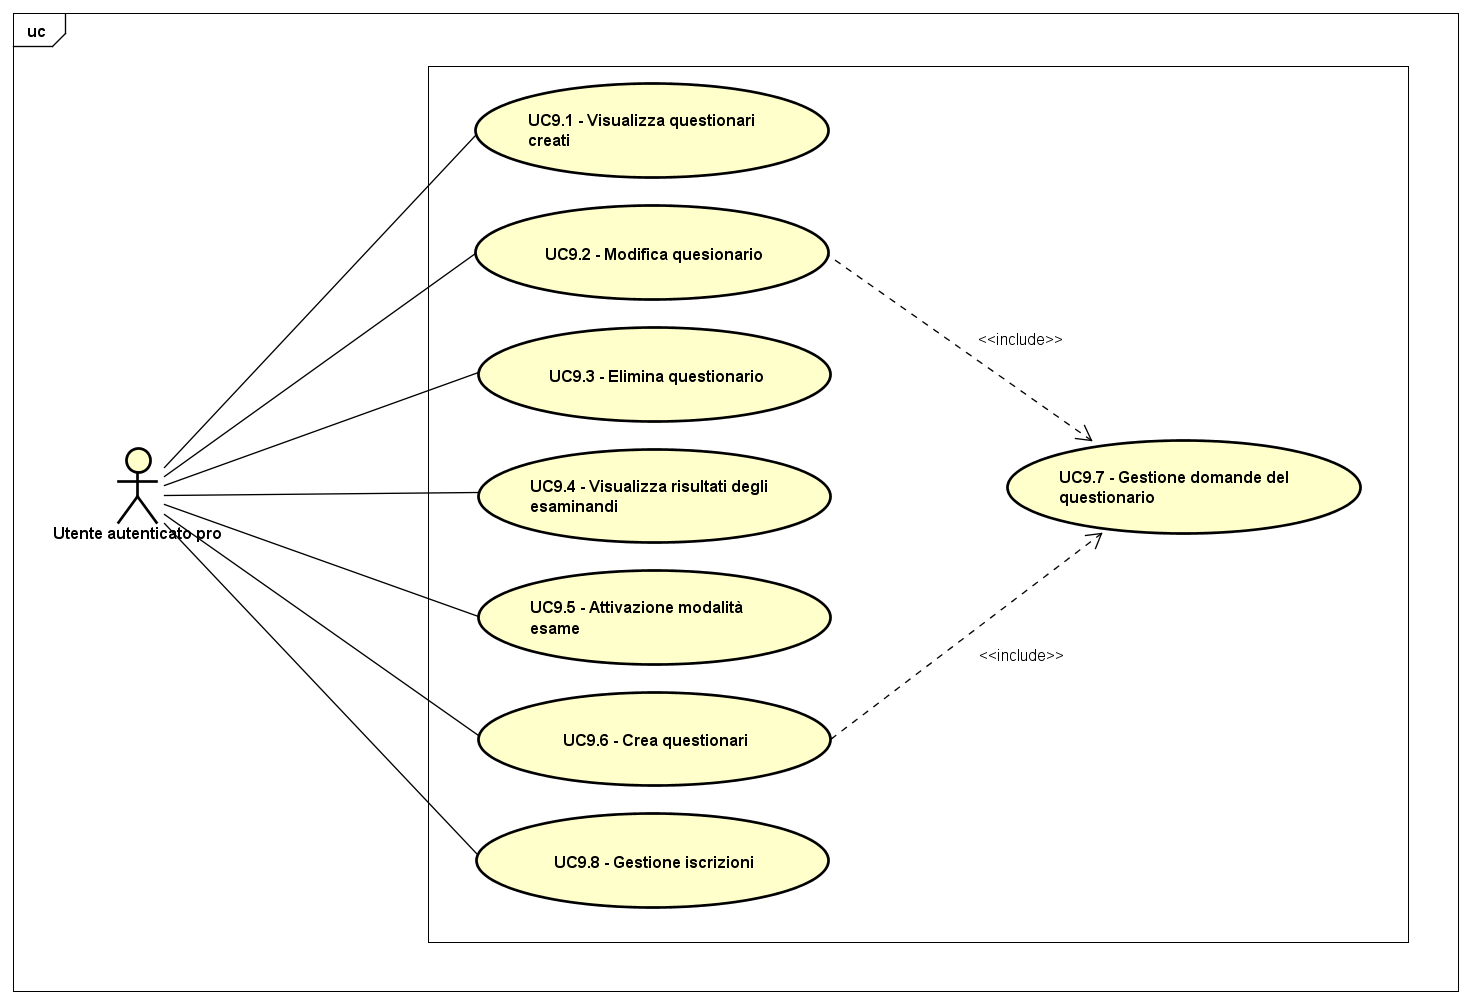
\includegraphics[scale=0.7,keepaspectratio]{UML/UC9.png}
				\caption{UC9.2: Cambia tipologia utente}
			\end{figure}
			\FloatBarrier
			\begin{itemize}
				\item \textbf{Attori}: 
				\item \textbf{Descrizione}: 
				\item \textbf{Precondizione}: 
				\item \textbf{Postcondizione}: 
				\item \textbf{Scenario principale}:
				\item \textbf{Inclusioni}:
				\item \textbf{Estensioni}:
				\item \textbf{Scenari alternativi}:
			\end{itemize}
			
		\paragraph{Caso d'uso UC9.2.2: Inserisci nome questionario}
		\label{UC9.2.2}
		\begin{figure}[h]
			\centering
		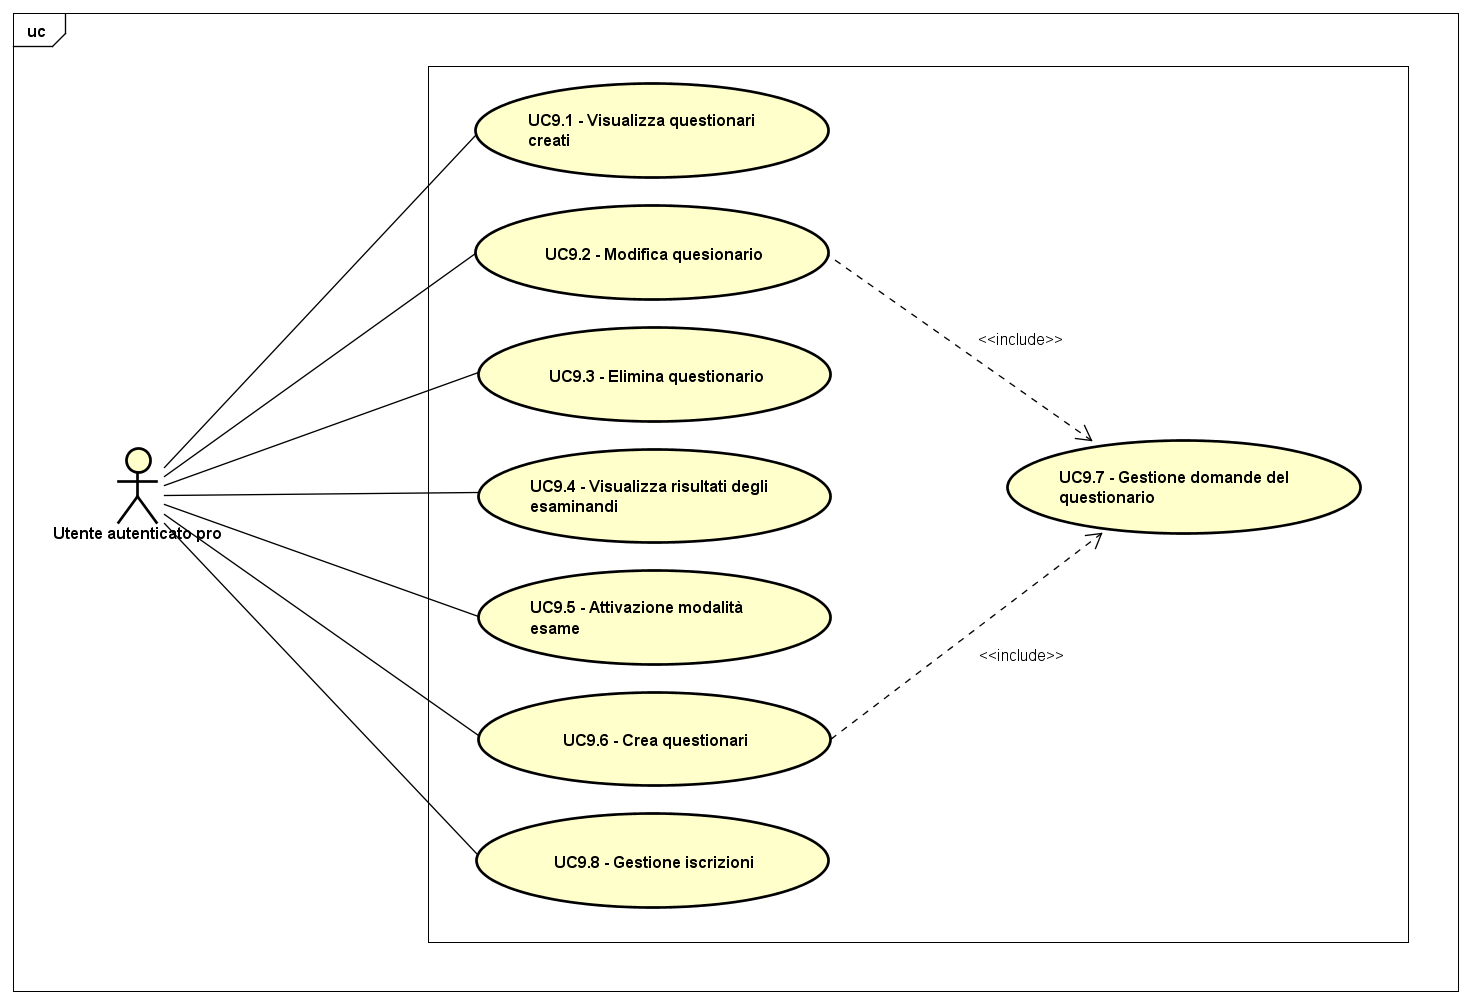
\includegraphics[scale=0.7,keepaspectratio]{UML/UC9.png}
			\caption{UC9.2.2: Inserisci nome questionario}
		\end{figure}
		\FloatBarrier
		\begin{itemize}
			\item \textbf{Attori}: 
			\item \textbf{Descrizione}: 
			\item \textbf{Precondizione}: 
			\item \textbf{Postcondizione}: 
			\item \textbf{Scenario principale}:
			\item \textbf{Inclusioni}:
			\item \textbf{Estensioni}:
			\item \textbf{Scenari alternativi}:
		\end{itemize}
		
		\paragraph{Caso d'uso UC9.2.3: Seleziona categorie questionario}
		\label{UC9.2.3}
		\begin{figure}[h]
			\centering
		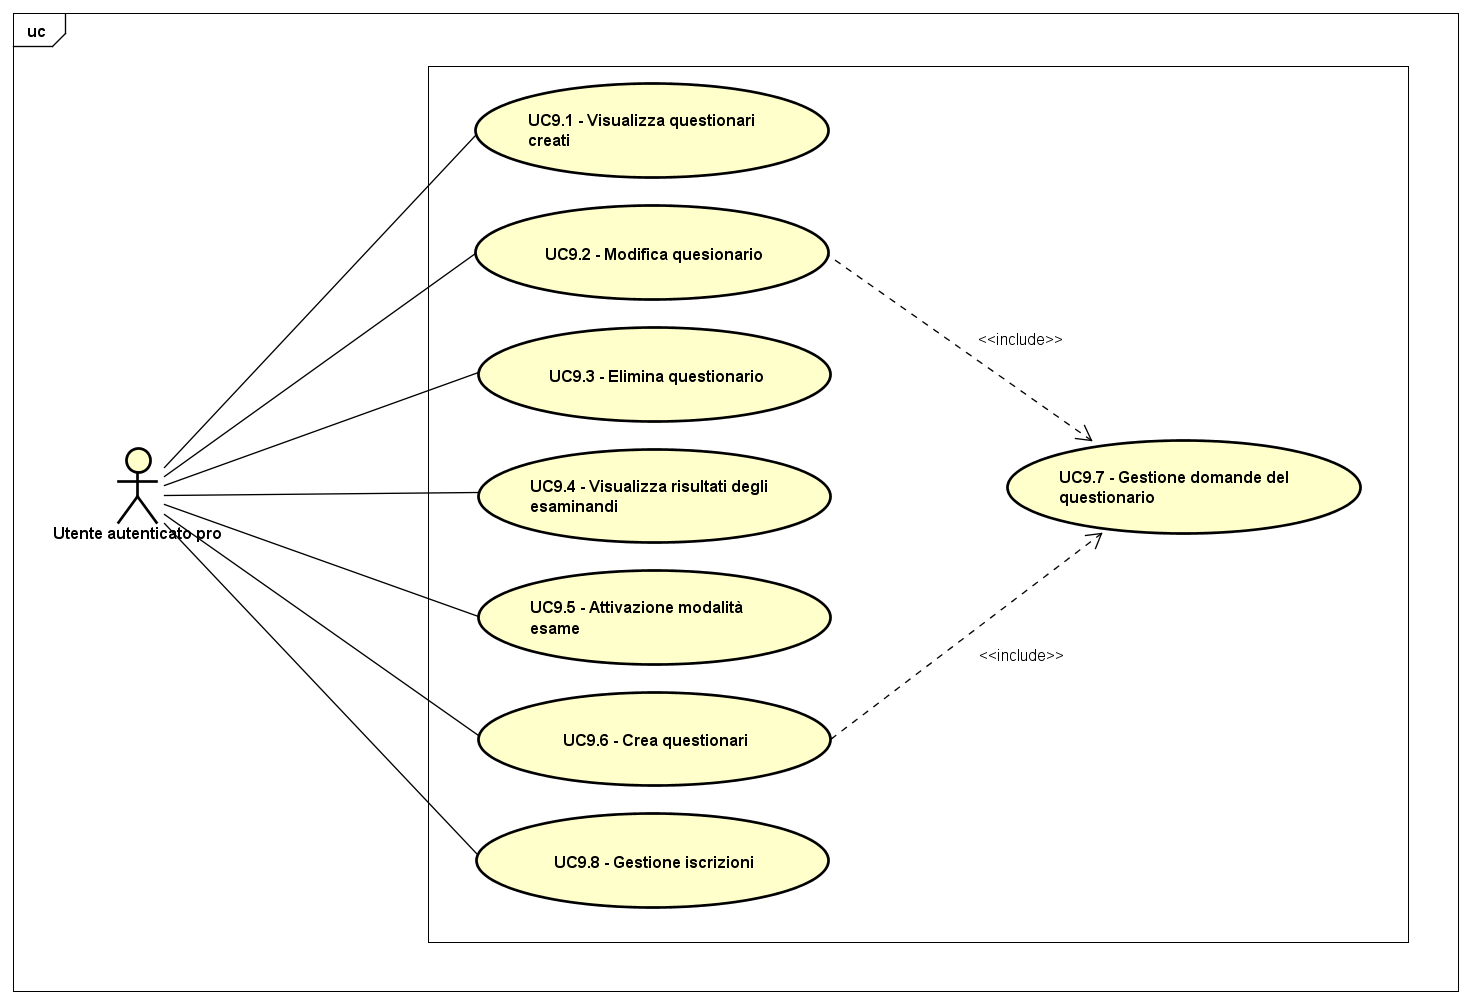
\includegraphics[scale=0.7,keepaspectratio]{UML/UC9.png}
			\caption{UC9.2.3: Seleziona categorie questionario}
		\end{figure}
		\FloatBarrier
		\begin{itemize}
			\item \textbf{Attori}: 
			\item \textbf{Descrizione}: 
			\item \textbf{Precondizione}: 
			\item \textbf{Postcondizione}: 
			\item \textbf{Scenario principale}:
			\item \textbf{Inclusioni}:
			\item \textbf{Estensioni}:
			\item \textbf{Scenari alternativi}:
		\end{itemize}
		
			\subparagraph{Caso d'uso UC9.2.3.1: Crea categoria}
			\label{UC9.2.3.1}
			\begin{figure}[h]
				\centering
			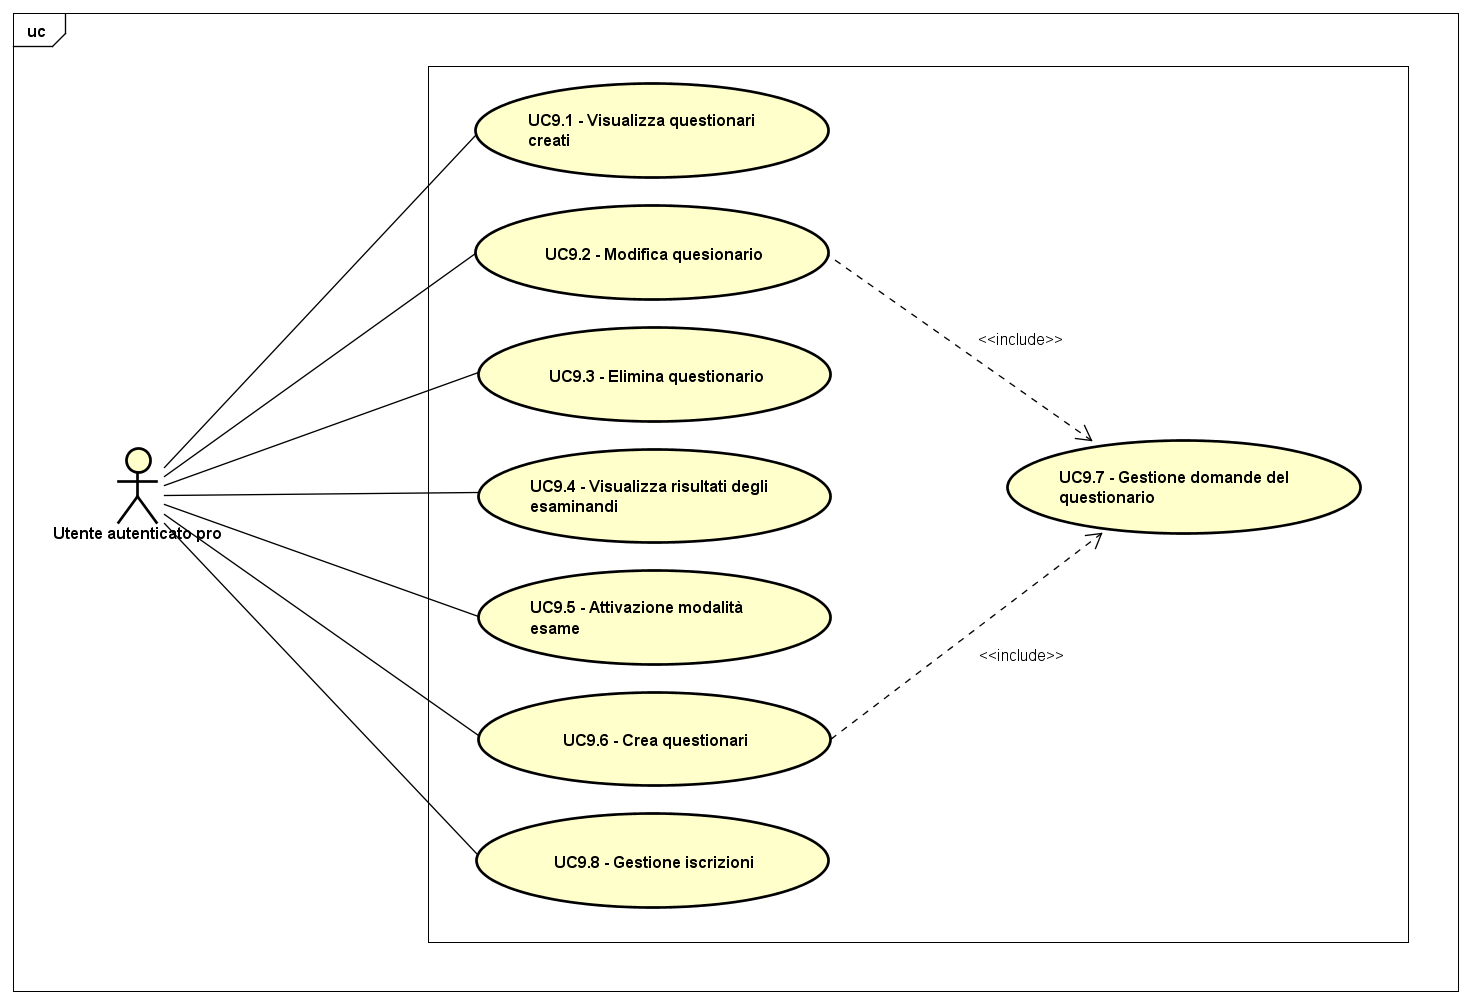
\includegraphics[scale=0.7,keepaspectratio]{UML/UC9.png}
				\caption{UC9.2.3.1: Crea categoria}
			\end{figure}
			\FloatBarrier
			\begin{itemize}
				\item \textbf{Attori}: 
				\item \textbf{Descrizione}: 
				\item \textbf{Precondizione}: 
				\item \textbf{Postcondizione}: 
				\item \textbf{Scenario principale}:
				\item \textbf{Inclusioni}:
				\item \textbf{Estensioni}:
				\item \textbf{Scenari alternativi}:
			\end{itemize}
			
		\paragraph{Caso d'uso UC9.2.4: Gestione domande}
		\label{UC9.2.4}
		\begin{figure}[h]
			\centering
		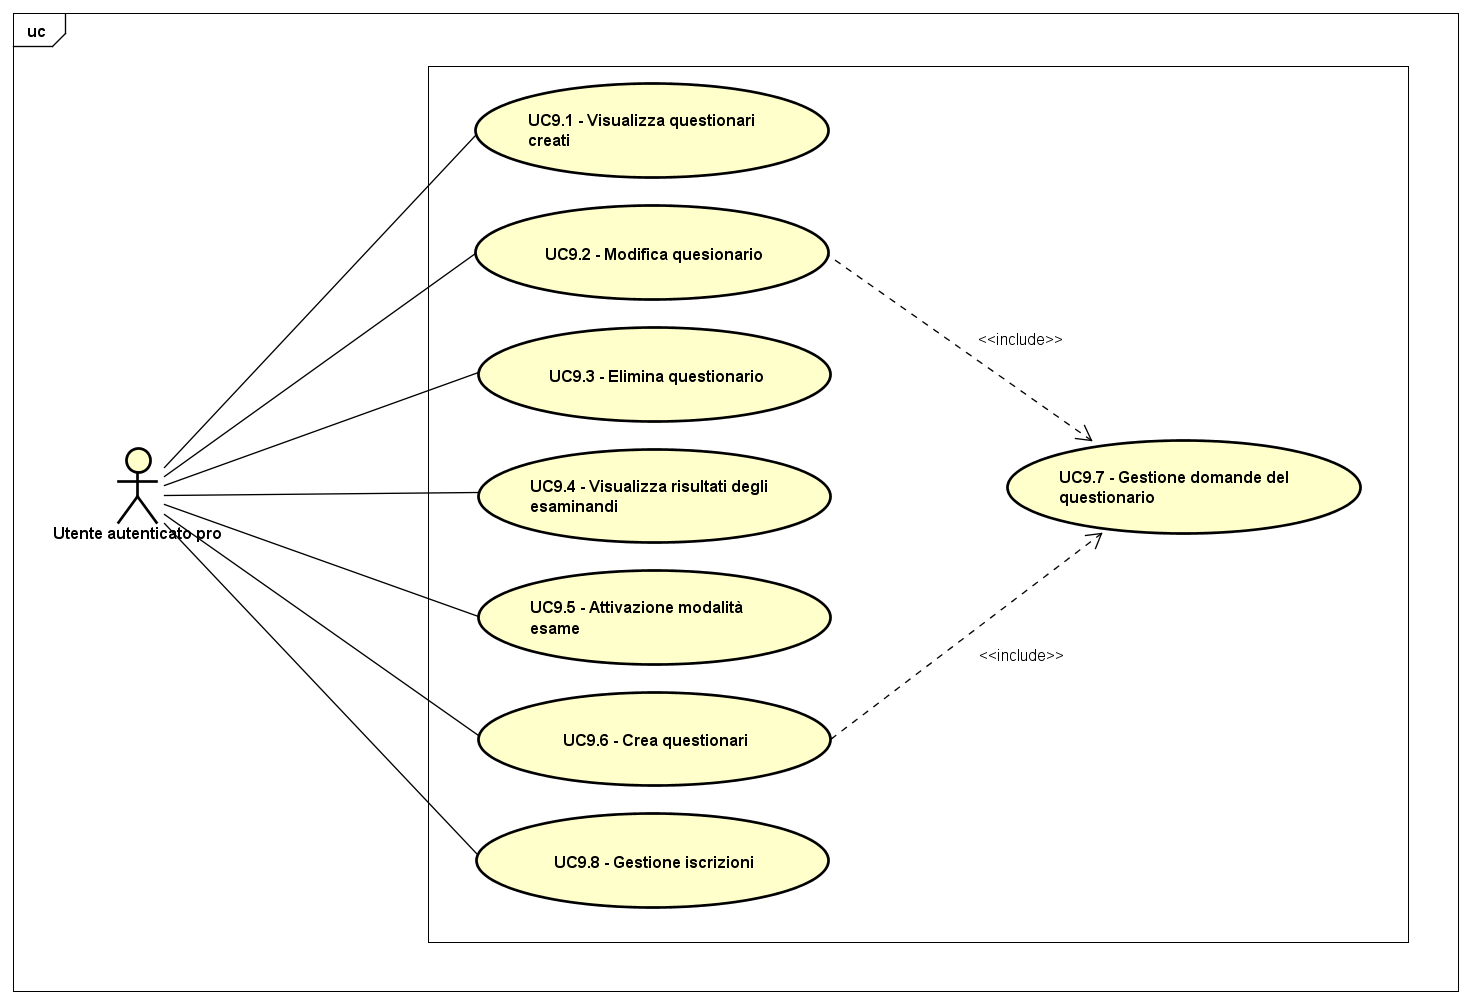
\includegraphics[scale=0.7,keepaspectratio]{UML/UC9.png}
			\caption{UC9.2.4: Gestione domande}
		\end{figure}
		\FloatBarrier
		\begin{itemize}
			\item \textbf{Attori}: 
			\item \textbf{Descrizione}: 
			\item \textbf{Precondizione}: 
			\item \textbf{Postcondizione}: 
			\item \textbf{Scenario principale}:
			\item \textbf{Inclusioni}:
			\item \textbf{Estensioni}:
			\item \textbf{Scenari alternativi}:
		\end{itemize}
		
			\subparagraph{Caso d'uso UC9.2.4.1: Genera automaticamente domande}
			\label{UC9.2.4.1}
			\begin{figure}[h]
				\centering
			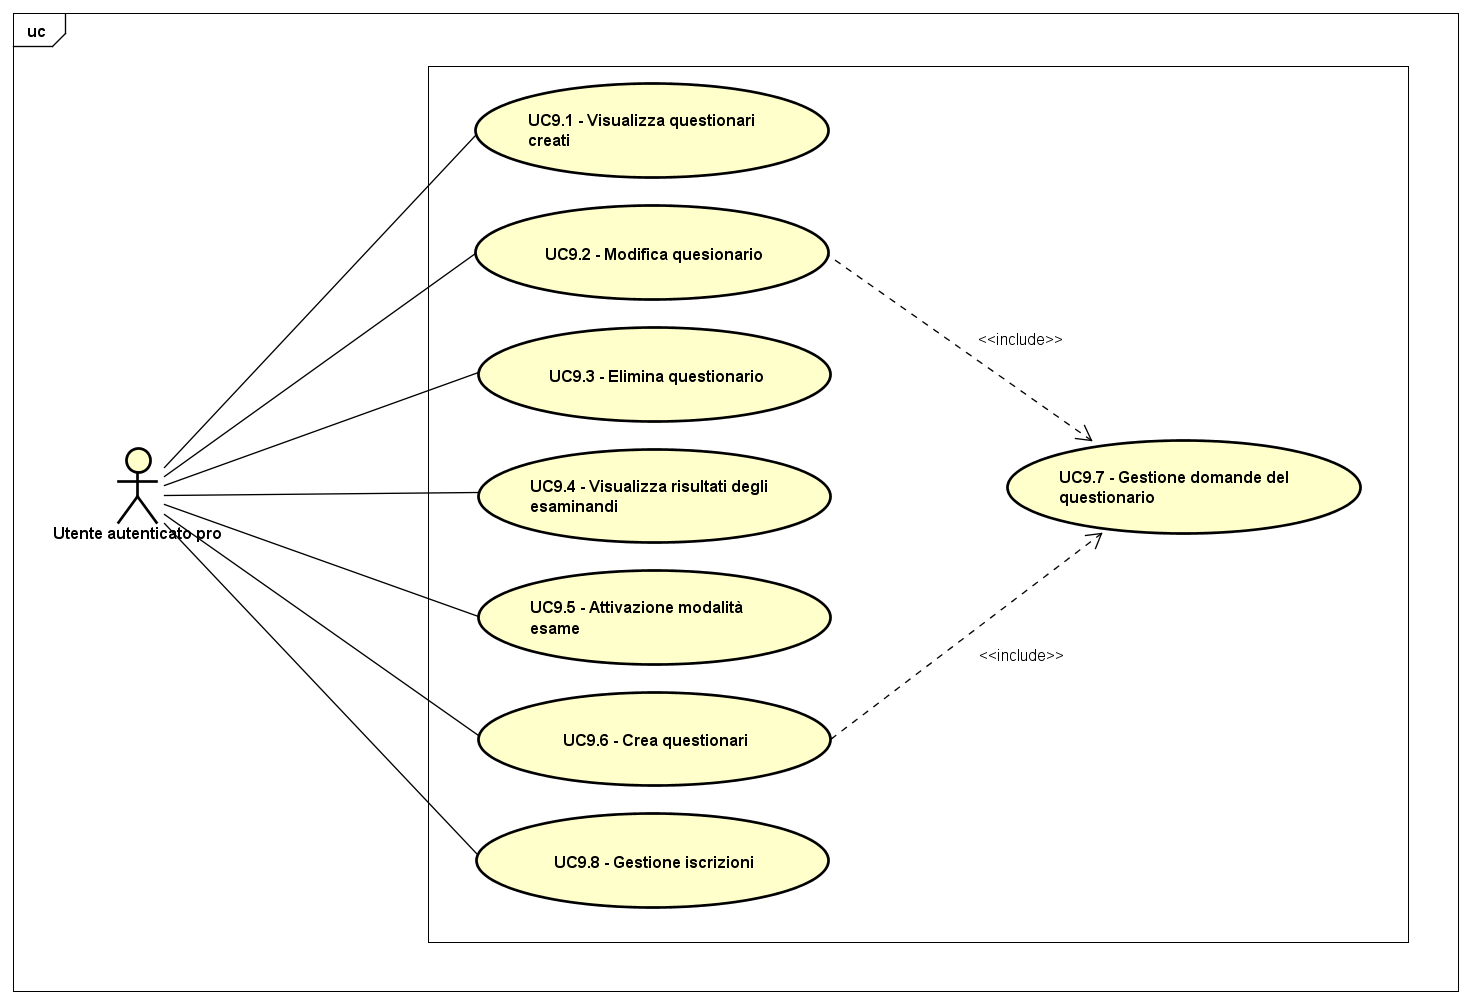
\includegraphics[scale=0.7,keepaspectratio]{UML/UC9.png}
				\caption{UC9.2.4.1: Genera automaticamente domande}
			\end{figure}
			\FloatBarrier
			\begin{itemize}
				\item \textbf{Attori}: 
				\item \textbf{Descrizione}: 
				\item \textbf{Precondizione}: 
				\item \textbf{Postcondizione}: 
				\item \textbf{Scenario principale}:
				\item \textbf{Inclusioni}:
				\item \textbf{Estensioni}:
				\item \textbf{Scenari alternativi}:
			\end{itemize}
			
			\subparagraph{Caso d'uso UC9.2.4.2: Seleziona domande}	
			\label{UC9.2.4.2}
			\begin{figure}[h]
				\centering
			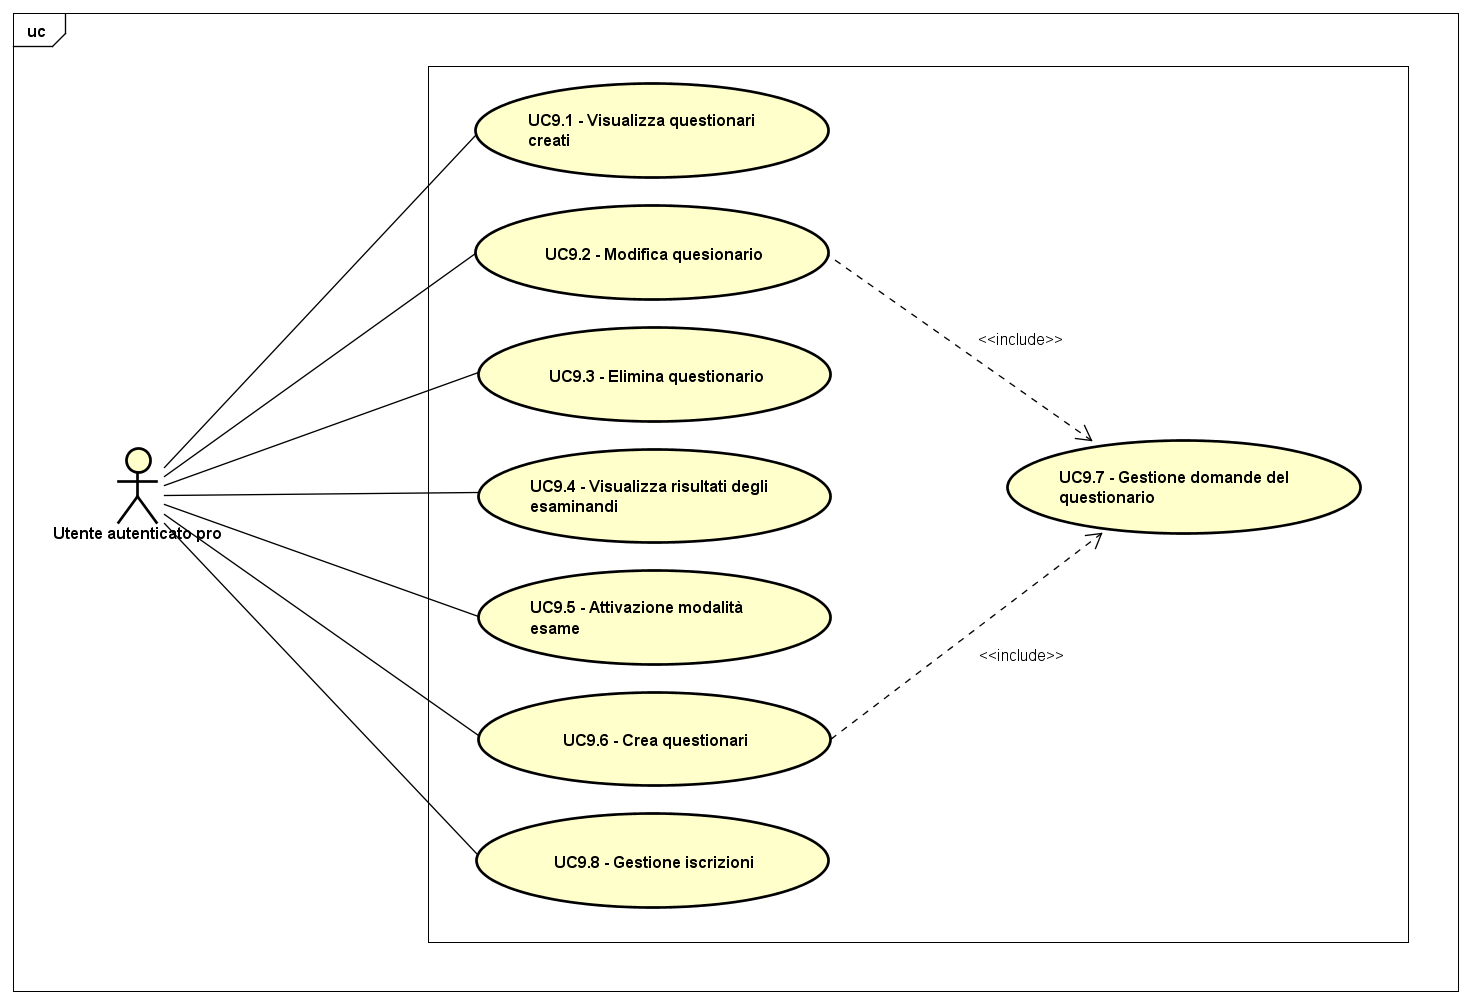
\includegraphics[scale=0.7,keepaspectratio]{UML/UC9.png}
				\caption{UC9.2.4.2: Seleziona domande}
			\end{figure}
			\FloatBarrier
			\begin{itemize}
				\item \textbf{Attori}: 
				\item \textbf{Descrizione}: 
				\item \textbf{Precondizione}: 
				\item \textbf{Postcondizione}: 
				\item \textbf{Scenario principale}:
				\item \textbf{Inclusioni}:
				\item \textbf{Estensioni}:
				\item \textbf{Scenari alternativi}:
			\end{itemize}
			
				\subsubparagraph{Caso d'uso UC9.2.4.2.1: Crea domanda}
				\label{UC9.2.4.2.1}
				\begin{figure}[h]
					\centering
				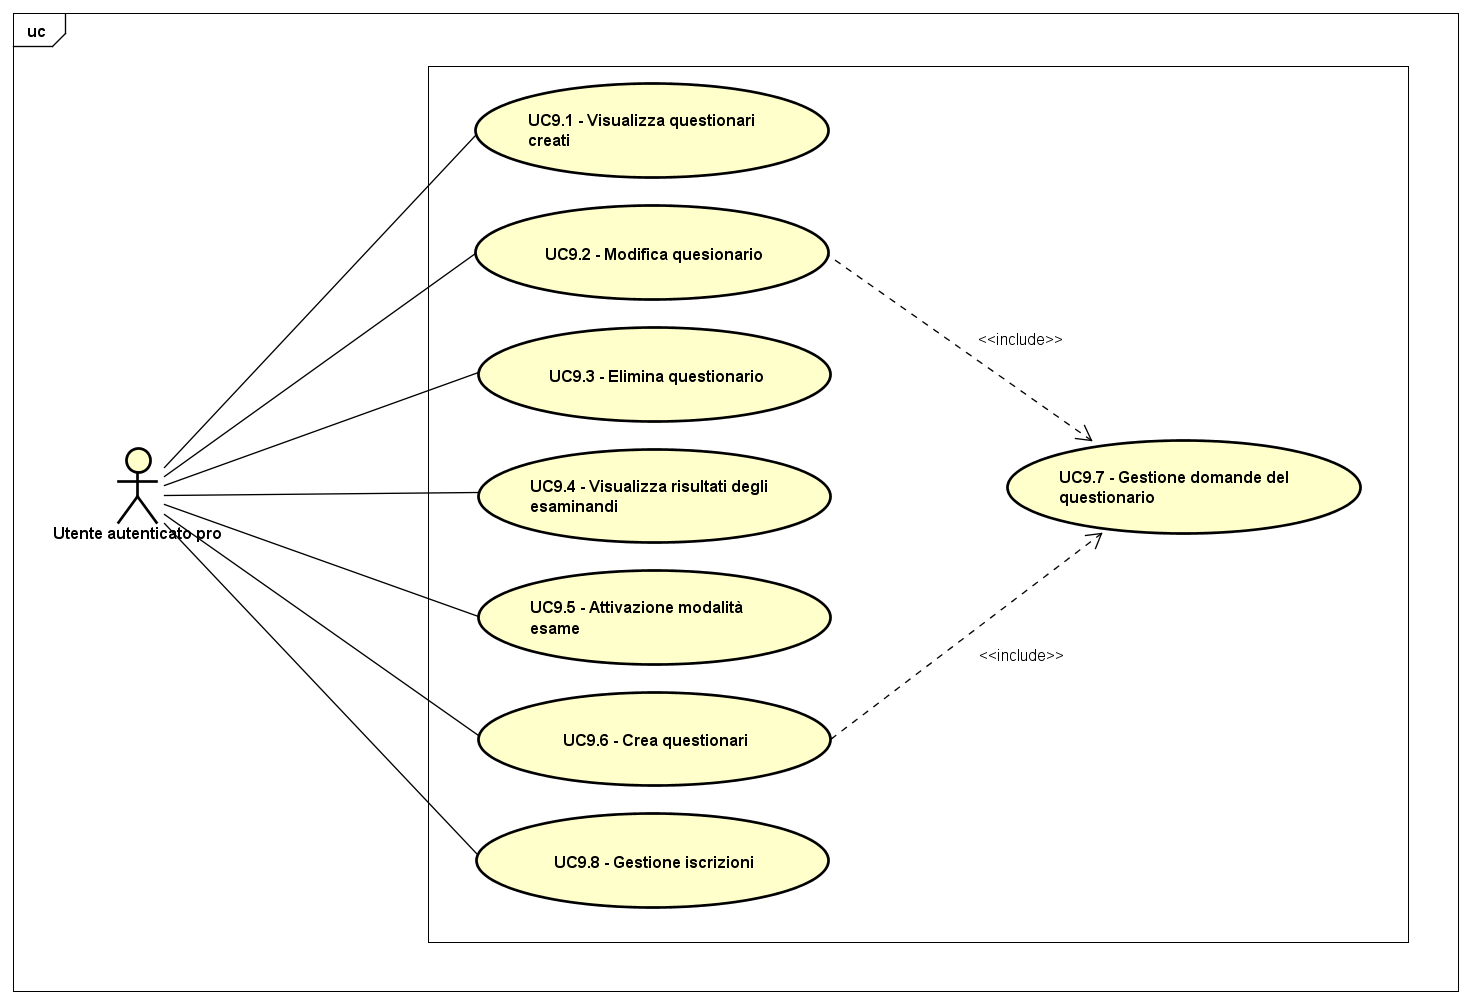
\includegraphics[scale=0.7,keepaspectratio]{UML/UC9.png}
					\caption{UC9.2.4.2.1: Crea domanda}
				\end{figure}
				\FloatBarrier
				\begin{itemize}
					\item \textbf{Attori}: 
					\item \textbf{Descrizione}: 
					\item \textbf{Precondizione}: 
					\item \textbf{Postcondizione}: 
					\item \textbf{Scenario principale}:
					\item \textbf{Inclusioni}:
					\item \textbf{Estensioni}:
					\item \textbf{Scenari alternativi}:
				\end{itemize}
				
		\paragraph{Caso d'uso UC9.2.5: Resoconto questionario}
		\label{UC9.2.5}
		\begin{figure}[h]
			\centering
		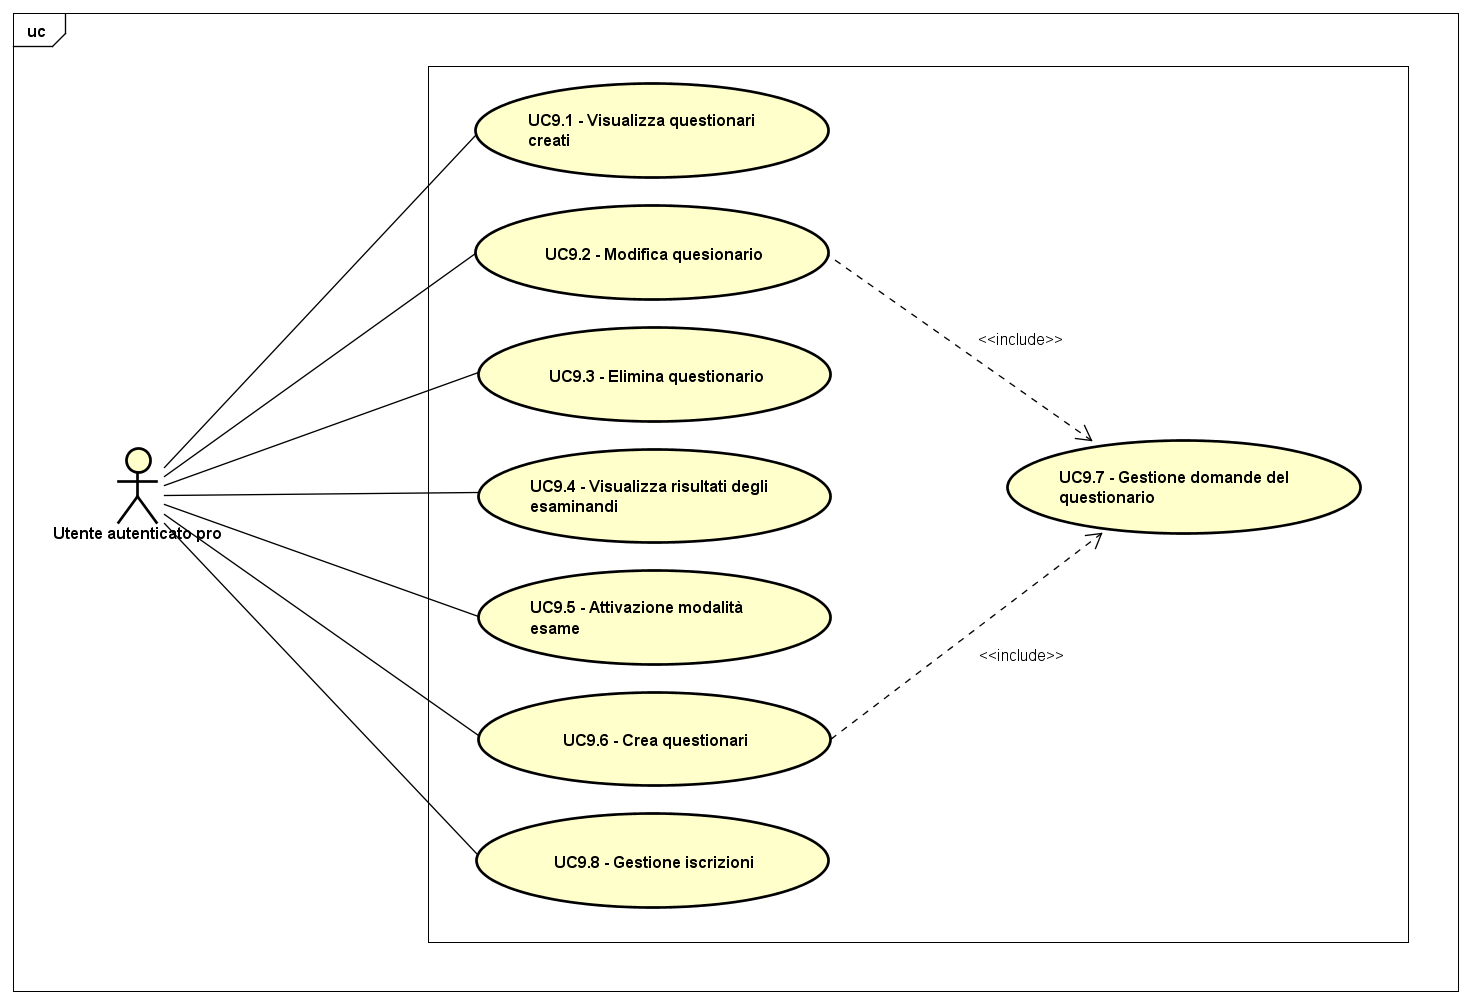
\includegraphics[scale=0.7,keepaspectratio]{UML/UC9.png}
			\caption{UC9.2.5: Resoconto questionario}
		\end{figure}
		\FloatBarrier
		\begin{itemize}
			\item \textbf{Attori}: 
			\item \textbf{Descrizione}: 
			\item \textbf{Precondizione}: 
			\item \textbf{Postcondizione}: 
			\item \textbf{Scenario principale}:
			\item \textbf{Inclusioni}:
			\item \textbf{Estensioni}:
			\item \textbf{Scenari alternativi}:
		\end{itemize}
		
		\paragraph{Caso d'uso UC9.2.6: Conferma questionario}
		\label{UC9.2.6}
		\begin{figure}[h]
			\centering
		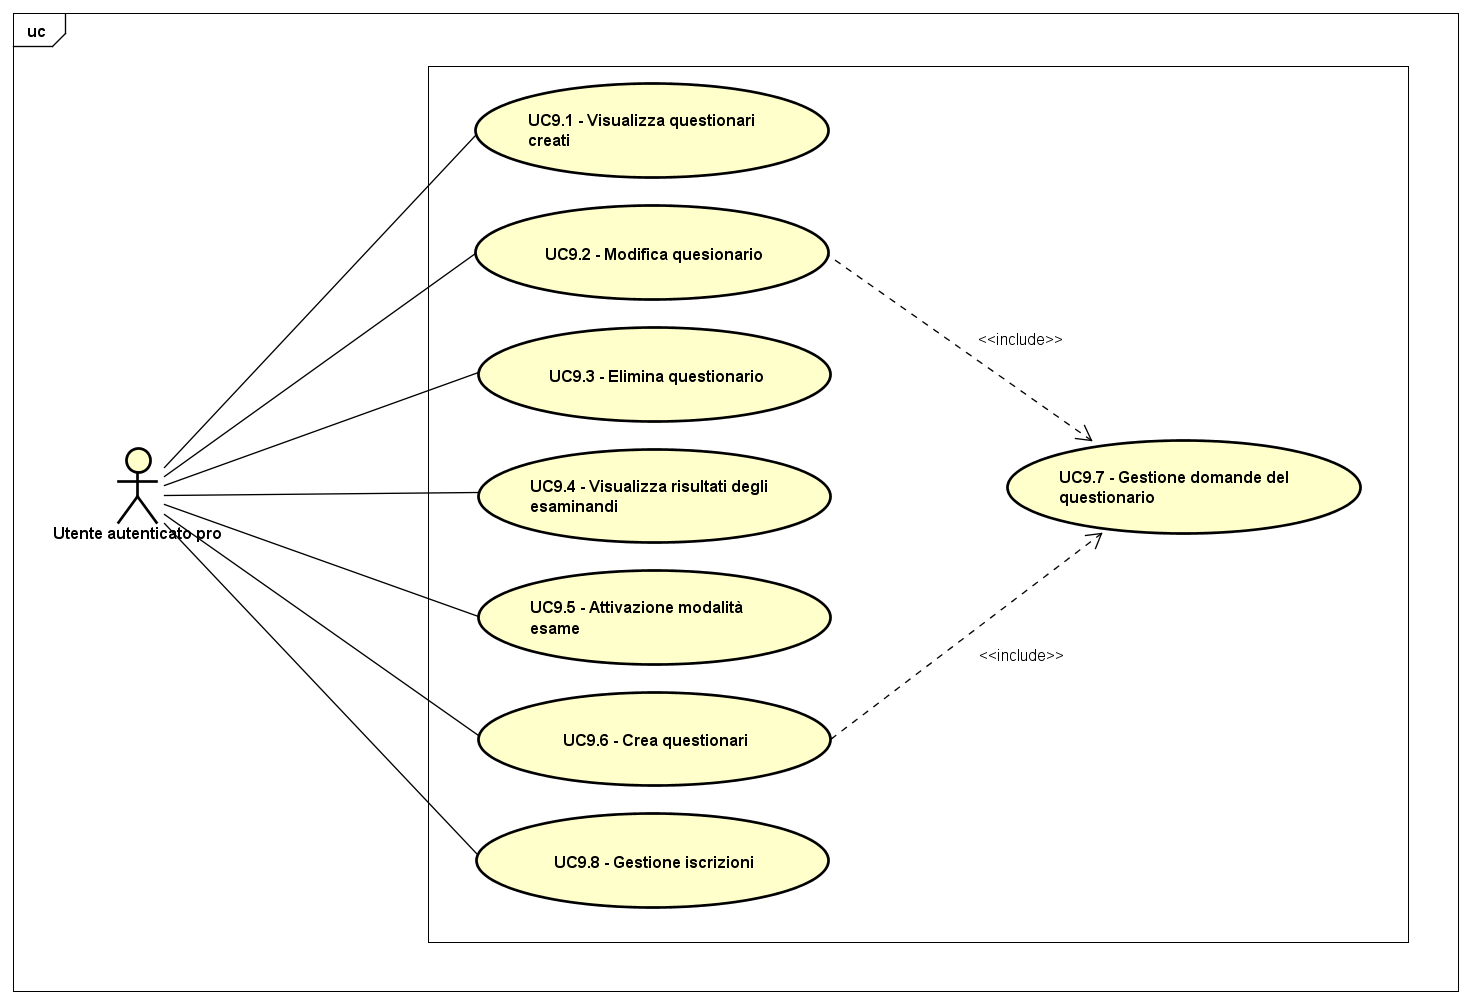
\includegraphics[scale=0.7,keepaspectratio]{UML/UC9.png}
			\caption{UC9.2.6: Conferma questionario}
		\end{figure}
		\FloatBarrier
		\begin{itemize}
			\item \textbf{Attori}: 
			\item \textbf{Descrizione}: 
			\item \textbf{Precondizione}: 
			\item \textbf{Postcondizione}: 
			\item \textbf{Scenario principale}:
			\item \textbf{Inclusioni}:
			\item \textbf{Estensioni}:
			\item \textbf{Scenari alternativi}:
		\end{itemize}
		
		\paragraph{Caso d'uso UC9.2.7: Annulla questionario}
		\label{UC9.2.7}
		\begin{figure}[h]
			\centering
		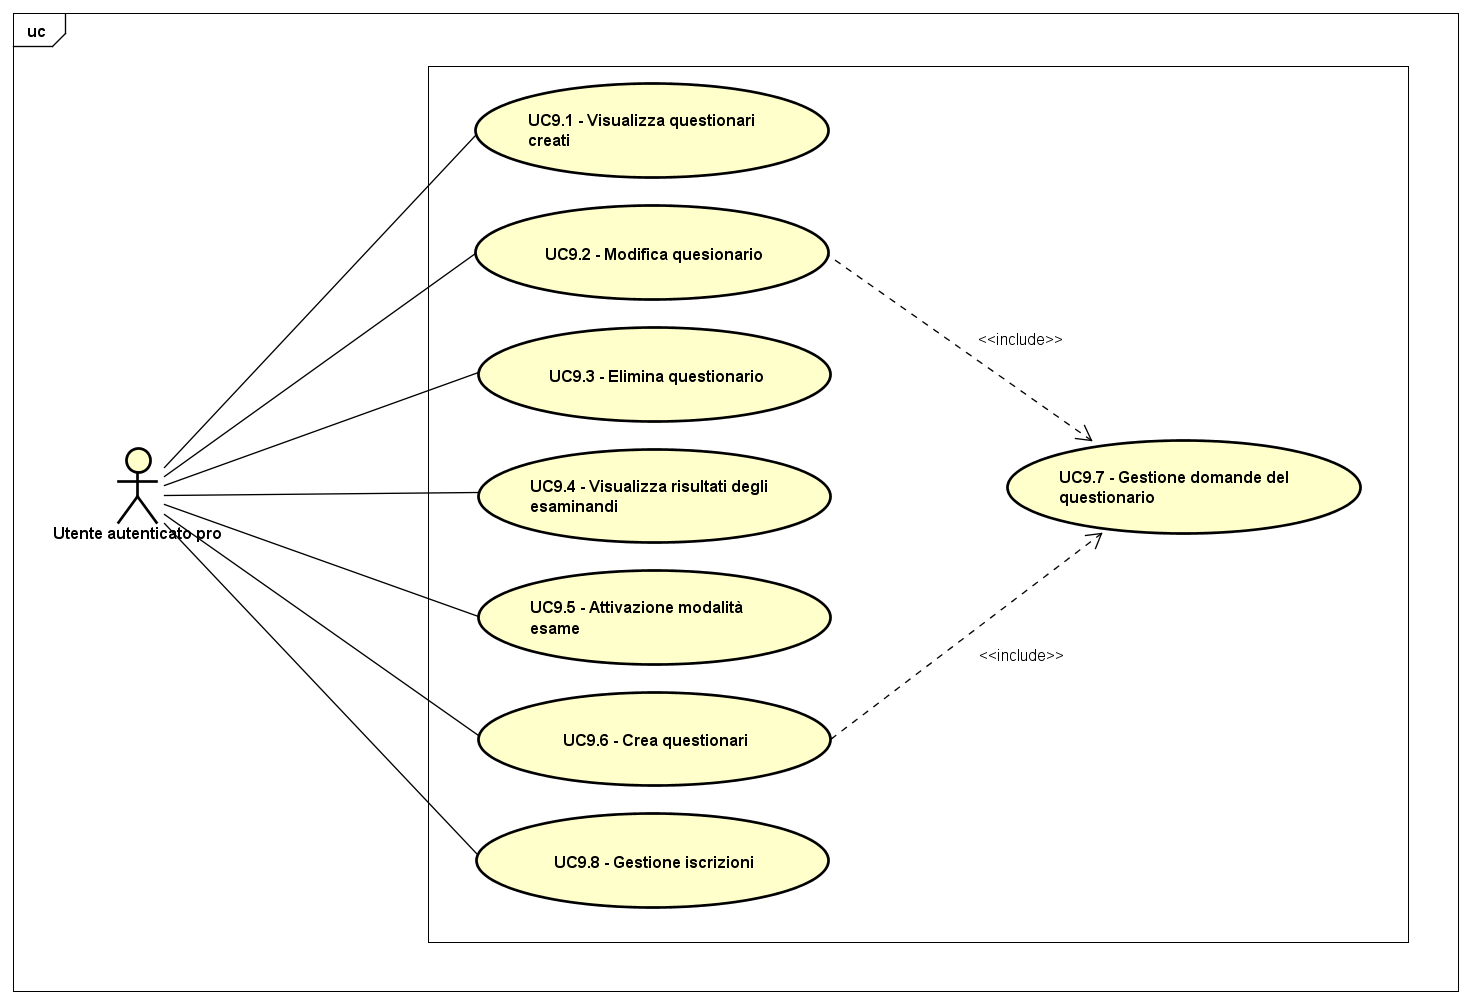
\includegraphics[scale=0.7,keepaspectratio]{UML/UC9.png}
			\caption{UC9.2.7: Annulla questionario}
		\end{figure}
		\FloatBarrier
		\begin{itemize}
			\item \textbf{Attori}: 
			\item \textbf{Descrizione}: 
			\item \textbf{Precondizione}: 
			\item \textbf{Postcondizione}: 
			\item \textbf{Scenario principale}:
			\item \textbf{Inclusioni}:
			\item \textbf{Estensioni}:
			\item \textbf{Scenari alternativi}:
		\end{itemize}

		